\documentclass[mathserif,serif]{beamer}

\usepackage[brazil]{babel}
\usepackage[utf8]{inputenc}

\usepackage{graphicx}
\usepackage{caption}
\usepackage{subcaption}
\usepackage{multimedia}
\usepackage{hyperref}
\usepackage{ragged2e}
\usepackage[none]{hyphenat}

\usetheme{CambridgeUS}
\usecolortheme{dolphin}
\setbeamertemplate{blocks}[rounded][shadow=false]

\title[]{Alocação de Tarefas para Transporte de Objetos com Robôs Heterogêneos}
\author[Ramon Soares de Melo]{
Ramon Soares de Melo\\
\vspace{0.8cm}
Douglas Guimarães Macharet\\
Mario Fernando Montenegro Campos\\
}
\institute[]
{
    
\includegraphics[height=0.1\textheight]{imgs/verlab.jpg}
    \hspace{0.4cm}
    
\includegraphics[height=0.1\textheight]{imgs/ppgcc.png}
    \hspace{0.4cm}
    
\includegraphics[height=0.1\textheight]{imgs/ufmg.png}\\
  % Instituto de Ciências Exatas - ICEx\\
  % Laboratório de Visão Computacional e Robótica - VerLab\\
  % Universidade Federal de Minas Gerais
  \vspace{0.8cm}
  {\large Defesa de Mestrado em Ciência da Computação}
}
\date{}
\subject{Computer Science}

% \movie[height=0.6\textwidth,width=\textwidth, autostart, loop, showcontrols=true]{}{newvideo.ogv}

\newcommand{\backupbegin}{
   \newcounter{framenumberappendix}
   \setcounter{framenumberappendix}{\value{framenumber}}
}
\newcommand{\backupend}{
   \addtocounter{framenumberappendix}{-\value{framenumber}}
   \addtocounter{framenumber}{\value{framenumberappendix}}
}

\begin{document}

    
\newcommand{\mrs}{MRS}
\newcommand{\environment}{\ensuremath{\mathbb{R}^3}}

% Shortcut definitions

\newcommand{\set}[1]{\ensuremath{\boldsymbol{\mathcal{#1}}}}
\newcommand{\setitem}[2]{\ensuremath{#1_{#2}}}
\newcommand{\setlist}[3]{#1\ $=$\ \{\setitem{#2}{1}, \setitem{#2}{2}, ..., \setitem{#2}{#3}\}}

\newcommand{\robotset}{\set{R}} % conjunto de robôs
\newcommand{\robotsetqt}{\ensuremath{k}}
\newcommand{\robot}[1]{\setitem{r}{#1}}
\newcommand{\robotlist}{\setlist{\robotset}{r}{\robotsetqt}}

\newcommand{\obstacleset}{\set{B}} % conjunto de obstáculos
\newcommand{\obstaclesetqt}{\ensuremath{x}}
\newcommand{\obstacle}[1]{\setitem{b}{#1}}
\newcommand{\obstaclelist}{\setlist{\obstacleset}{b}{\obstaclesetqt}}

\newcommand{\objectset}{\set{O}} % conjunto de objetos
\newcommand{\objectsetqt}{\ensuremath{y}}
\newcommand{\object}[1]{\setitem{o}{#1}}
\newcommand{\objectlist}{\setlist{\objectset}{o}{\objectsetqt}}

\newcommand{\planset}{\set{P}} % plano
\newcommand{\plansetqt}{\ensuremath{q}}
\newcommand{\plan}[1]{\setitem{n}{#1}}
\newcommand{\planlist}{\setlist{\planset}{n}{\plansetqt}}

\newcommand{\robotplanset}{\set{RP}} % conjunto de planos
\newcommand{\robotplansetqt}{\ensuremath{j}}
\newcommand{\robotplan}[1]{\setitem{rp}{#1}}
\newcommand{\robotplanlist}{\setlist{\robotplanset}{rp}{\robotplansetqt}}

\newcommand{\executionplanset}{\set{EP}} % conjunto de planos
\newcommand{\executionplansetqt}{\ensuremath{h}}
\newcommand{\executionplan}[1]{\setitem{ep}{#1}}
\newcommand{\executionplanlist}{\setlist{\executionplanset}{ep}{\executionplansetqt}}
\newcommand{\executionplanname}{\emph{Execution Plan}}
\newcommand{\executionplansetnotation}{\ensuremath{\executionplanset \subset \robotplanset}}

\newcommand{\executionplanminset}{\ensuremath{\executionplanset{*}}} % conjunto com custo minimo de segmentos

\newcommand{\segmentset}{\set{S}} % conjunto de segmentos
\newcommand{\segmentsetqt}{\ensuremath{e}}
\newcommand{\segment}[1]{\setitem{s}{#1}}
\newcommand{\segmentlist}{\setlist{\segmentset}{s}{\segmentsetqt}}

\newcommand{\segmentpointset}{\ensuremath{\set{S}_p}} % conjunto de pontos de segmentação
\newcommand{\segmentpointsetqt}{\ensuremath{z}}
\newcommand{\segmentpoint}[1]{\setitem{sp}{#1}}
\newcommand{\segmentpointfirst}[1]{\ensuremath{\segmentpoint{#1}^1}}
\newcommand{\segmentpointsecond}[1]{\ensuremath{\segmentpoint{#1}^2}}

\newcommand{\segmentpointlist}{\setlist{\segmentpointset}{sp}{\segmentpointsetqt}}

\newcommand{\typeland}{ground}
\newcommand{\typeaerial}{aerial}
\newcommand{\typeset}{\set{T}} % conjunto de tipos de movimentação
\newcommand{\typelist}{\ensuremath{\typeset=\ \{}\typeland, \typeaerial\ensuremath{\}}}
\newcommand{\type}[1]{\setitem{t}{#1}}

\newcommand{\plantypestart}{initial}
\newcommand{\plantypetransition}{transition}
\newcommand{\plantypemove}{movement}
\newcommand{\plantypeset}{\set{TP}} % conjunto de tipos de plano
\newcommand{\plantypelist}{\ensuremath{\plantypeset=\ \{}\plantypestart, \plantypetransition, \plantypemove\ensuremath{\}}}
\newcommand{\plantype}[1]{\setitem{tp}{#1}}

\newcommand{\movementtypepremove}{pre-transport}
\newcommand{\movementtypemove}{transport}
\newcommand{\movementtypeset}{\set{T_m}} % conjunto de tipos de plano
\newcommand{\movementtypelist}{\ensuremath{\movementtypeset=\ \{}\movementtypepremove, \movementtypemove\ensuremath{\}}}
\newcommand{\movementtype}[1]{\setitem{tm}{#1}}

\newcommand{\tokenset}{\set{TO}}
\newcommand{\tokensetqt}{\ensuremath{u}}
\newcommand{\tokeni}[1]{\setitem{to}{#1}}
\newcommand{\token}{\emph{token}}
\newcommand{\tokenlist}{\setlist{\tokenset}{to}{\tokensetqt}}

\newcommand{\workspace2}{\ensuremath{\boldsymbol{\mathcal{W}}}} % àrea de trabalho
\newcommand{\workspacecell}{\ensuremath{\boldsymbol{\mathcal{c}}}} % àrea de trabalho

\newcommand{\allocationgraph}{\ensuremath{\mathcal{AG}}}
\newcommand{\allocationgraphcompress}{\ensuremath{\mathcal{AG}_c}}

\newcommand{\currentstate}{\ensuremath{S}}
\newcommand{\nextstate}{\ensuremath{S'}}
\newcommand{\originstate}{\ensuremath{S_o}}
\newcommand{\targetstate}{\ensuremath{S_d}}
\newcommand{\robotstate}{\ensuremath{S_r}}

\newcommand{\robotinitialstate}{\ensuremath{I}}
\newcommand{\robotinitialstatei}[1]{\ensuremath{I_{#1}}}

\newcommand{\celldimension}{\ensuremath{d}}
\newcommand{\deslocationfactor}{\ensuremath{l}}

\newcommand{\movementset}{\set{M}}
\newcommand{\movementslist}{\ensuremath{\movementset=\ \{}left, right, front, back, up, down\ensuremath{\}}}
\newcommand{\movementaction}{\ensuremath{a_i}}

% Funções

\newcommand{\utilityfunction}{\ensuremath{\Theta}}
\newcommand{\utilityplanfunction}{\ensuremath{\utilityfunction_{p}}}
\newcommand{\utilitytotalfunction}{\ensuremath{\utilityfunction_{t}}}
\newcommand{\distancefunction}{\ensuremath{\Delta}}
\newcommand{\timefunction}{\ensuremath{\Upsilon}}
\newcommand{\energyfunction}{\ensuremath{\Psi}}

% Planejamento

\newcommand{\fringe}{\set{F}}
\newcommand{\searchednodes}{\set{SN}}
\newcommand{\node}{\ensuremath{n}}
\newcommand{\nodeitem}[1]{\ensuremath{\node_{#1}}}
\newcommand{\nodeparent}{\emph{NodePai}}
\newcommand{\nodeutility}{\ensuremath{\omega}}
\newcommand{\nodedata}{\ensuremath{\{}state (\currentstate), action (\movementaction), utility (\nodeutility), agent's position (\robotstate), type (\type{i})\ensuremath{\}}}


    \begin{frame}
        \titlepage
    \end{frame}

    % \begin{frame}
    %     \frametitle{Table of Contents}
    %     \tableofcontents[currentsection]
    % \end{frame}

    \section{Introdução} % (fold)
    \label{sec:introdu_o}

    \subsection{Contextualização} % (fold)

    \frame{
        \frametitle{Aplicações dos Robôs}

        \begin{figure}[p]
            \centering
            \setlength{\fboxsep}{0pt}
            \begin{subfigure}[b]{0.24\textwidth}
                \fbox{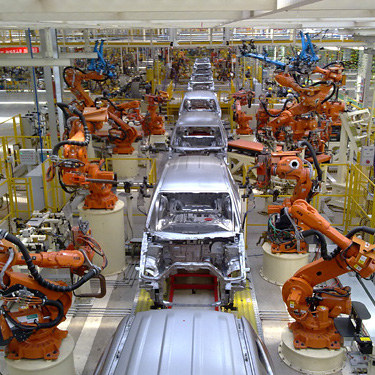
\includegraphics[width=\textwidth]{imgs/linha_montagem.jpg}}
                \caption*{Manufatura}
            \end{subfigure}
            \begin{subfigure}[b]{0.24\textwidth}
                \fbox{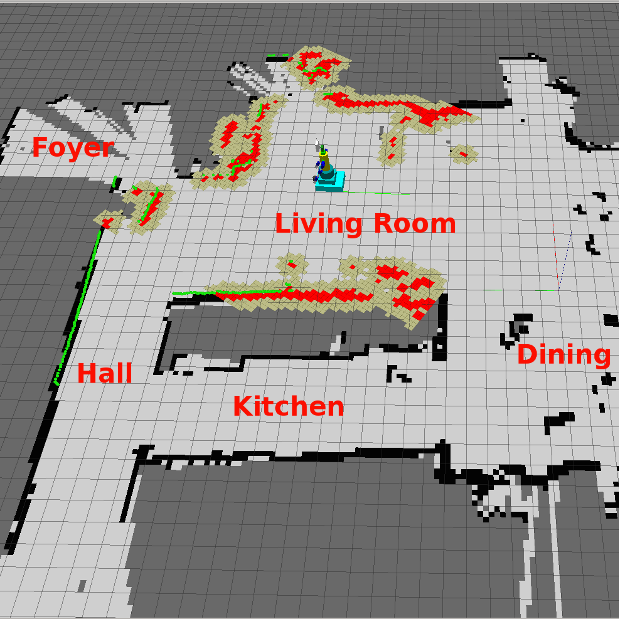
\includegraphics[width=\textwidth]{imgs/mapeamento.png}}
                \caption*{Mapeamento}
            \end{subfigure}
            \begin{subfigure}[b]{0.24\textwidth}
                \fbox{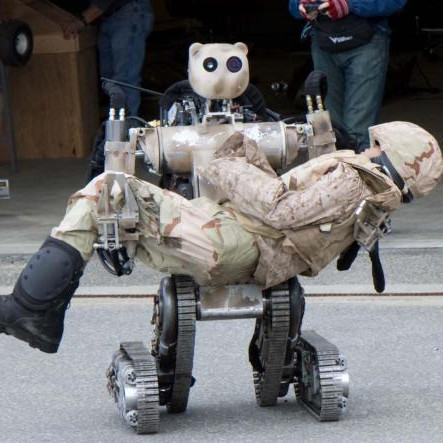
\includegraphics[width=\textwidth]{imgs/resgate.jpg}}
                \caption*{Resgate}
            \end{subfigure}\\
            \vspace{0.1cm}
            \begin{subfigure}[b]{0.24\textwidth}
                \fbox{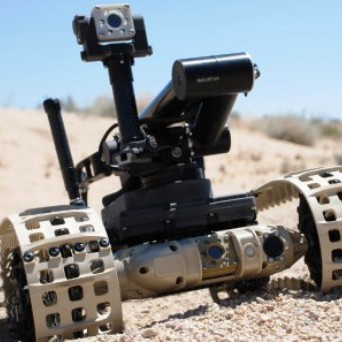
\includegraphics[width=\textwidth]{imgs/vigilancia.jpg}}
                \caption*{Vigilância}
            \end{subfigure}
            \begin{subfigure}[b]{0.24\textwidth}
                \fbox{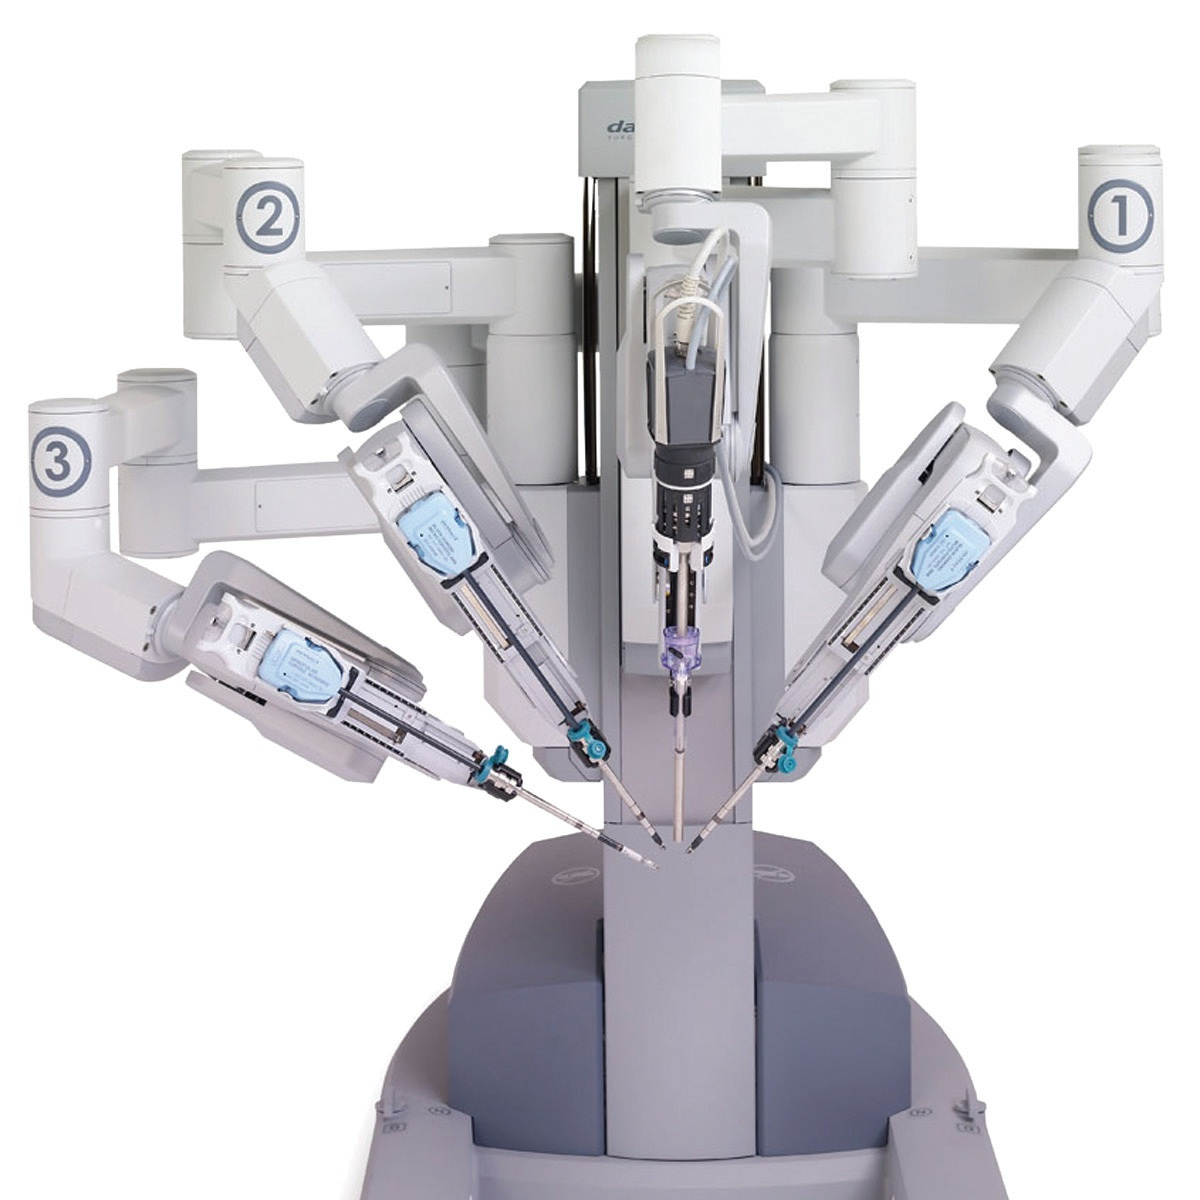
\includegraphics[width=\textwidth]{imgs/transporte3.jpg}}
                \caption*{Ferramentas}
            \end{subfigure}
            \begin{subfigure}[b]{0.24\textwidth}
                \fbox{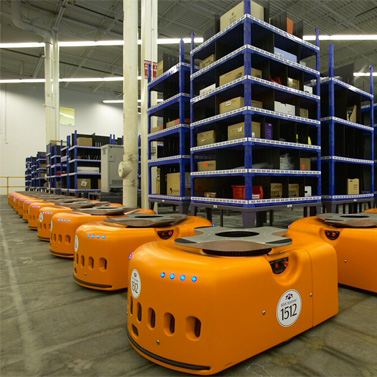
\includegraphics[width=\textwidth]{imgs/transporte1.png}}
                \caption*{Transporte}
            \end{subfigure}
        \end{figure}
    }

    % \frame{
        % OUT
        % \frametitle{Classificação quanto número de Agentes}
        % \begin{block}{Single Robot System -- SRS}
        %     Caso no qual a missão é planejada e executada utilizando somente um agente, que deve ser capaz de realizá-la completamente e possuir todas as capacidades necessárias.
        % \end{block}
        % \begin{block}{Multi Robot System -- MRS}
        %     Sistema munido de vários agentes disponíveis para realizar a tarefa, podendo cada agente possuir diferentes recursos e capacidades.
        % \end{block}
    % }

    \frame{
        \frametitle{Sistema Multi Robô}

        \begin{block}{Vantagens}
            \begin{itemize}
                \item Maior tolerância a falhas;
                \item Podem reduzir o tempo total de execução da tarefa;
                \item Executar tarefas complexas com agentes simples.
            \end{itemize}
        \end{block}

        \begin{block}{Dificuldades}
            \begin{itemize}
                \item Planejamento de Caminhos;
                \item Alocação de Tarefas;
                \item Coordenação.
            \end{itemize}
        \end{block}
    }

    \subsection{Motivação} % (fold)
    \label{sub:motiva_o}

    % \frame{
        % OUT
        % \frametitle{Manipulação de Objetos}

        % Transporte e manipulação de objetos é uma tarefa básica em diversas outras atividades:

        % \begin{figure}[p]
        %     \setlength{\fboxsep}{0pt}
        %     \centering
        %     \begin{subfigure}[b]{0.24\textwidth}
        %         \fbox{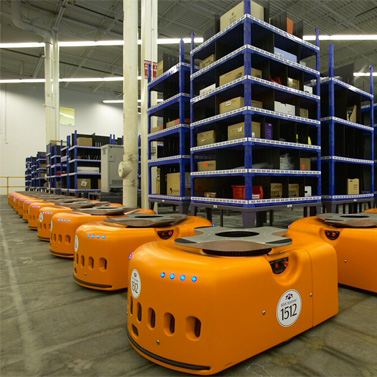
\includegraphics[width=\textwidth]{imgs/transporte1.png}}
        %         \caption*{Transporte}
        %     \end{subfigure}
        %     \begin{subfigure}[b]{0.24\textwidth}
        %         \fbox{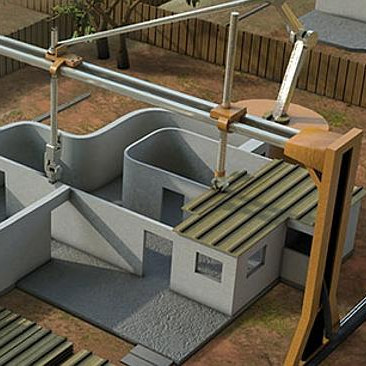
\includegraphics[width=\textwidth]{imgs/transporte2.jpg}}
        %         \caption*{Construção}
        %     \end{subfigure}
        %     \begin{subfigure}[b]{0.24\textwidth}
        %         \fbox{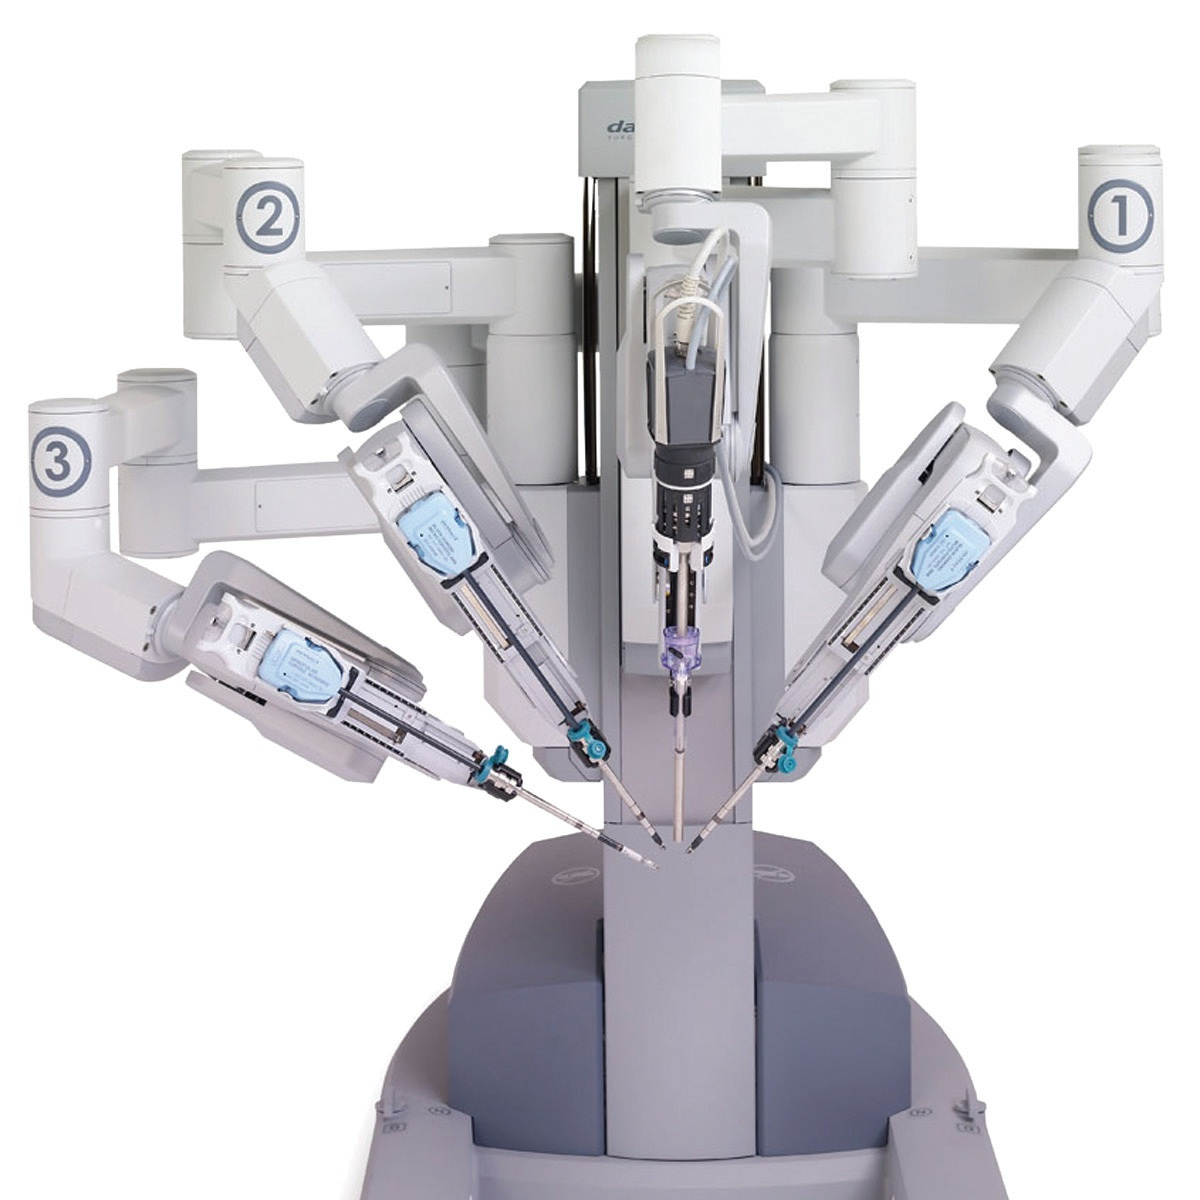
\includegraphics[width=\textwidth]{imgs/transporte3.jpg}}
        %         \caption*{Ferramentas}
        %     \end{subfigure}
        %     \begin{subfigure}[b]{0.24\textwidth}
        %         \fbox{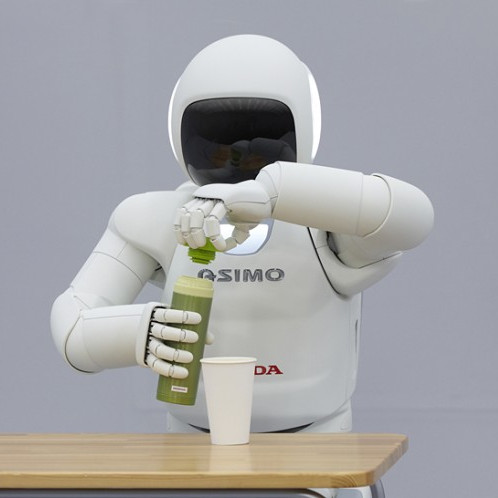
\includegraphics[width=\textwidth]{imgs/transporte4.jpg}}
        %         \caption*{Uso doméstico}
        %     \end{subfigure}

        % \end{figure}
    % }

    \frame{
        \frametitle{Tipo de Manipulação}

        \begin{columns}[T]
            \begin{column}[T]{0.5\textwidth}

                \begin{block}{Não-preênsil}
                    \justify
                    Agente utiliza ações como arremessar, rolar e empurrar para transportar o objeto.
                \end{block}

                \begin{figure}[p]
                    \centering
                    \setlength{\fboxsep}{0pt}
                    \fbox{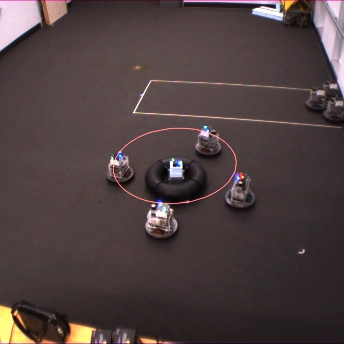
\includegraphics[width=0.6\textwidth]{imgs/fink.png}}
                    \caption*{\cite{Fink2008}}
                \end{figure}

            \end{column}
            \begin{column}[T]{0.5\textwidth}

                \begin{block}{Preênsil}
                    \justify
                    Agente utiliza um manipulador para acolher ou segurar o objeto a ser transportado.
                \end{block}

                \begin{figure}[p]
                    \centering
                    \setlength{\fboxsep}{0pt}
                    \fbox{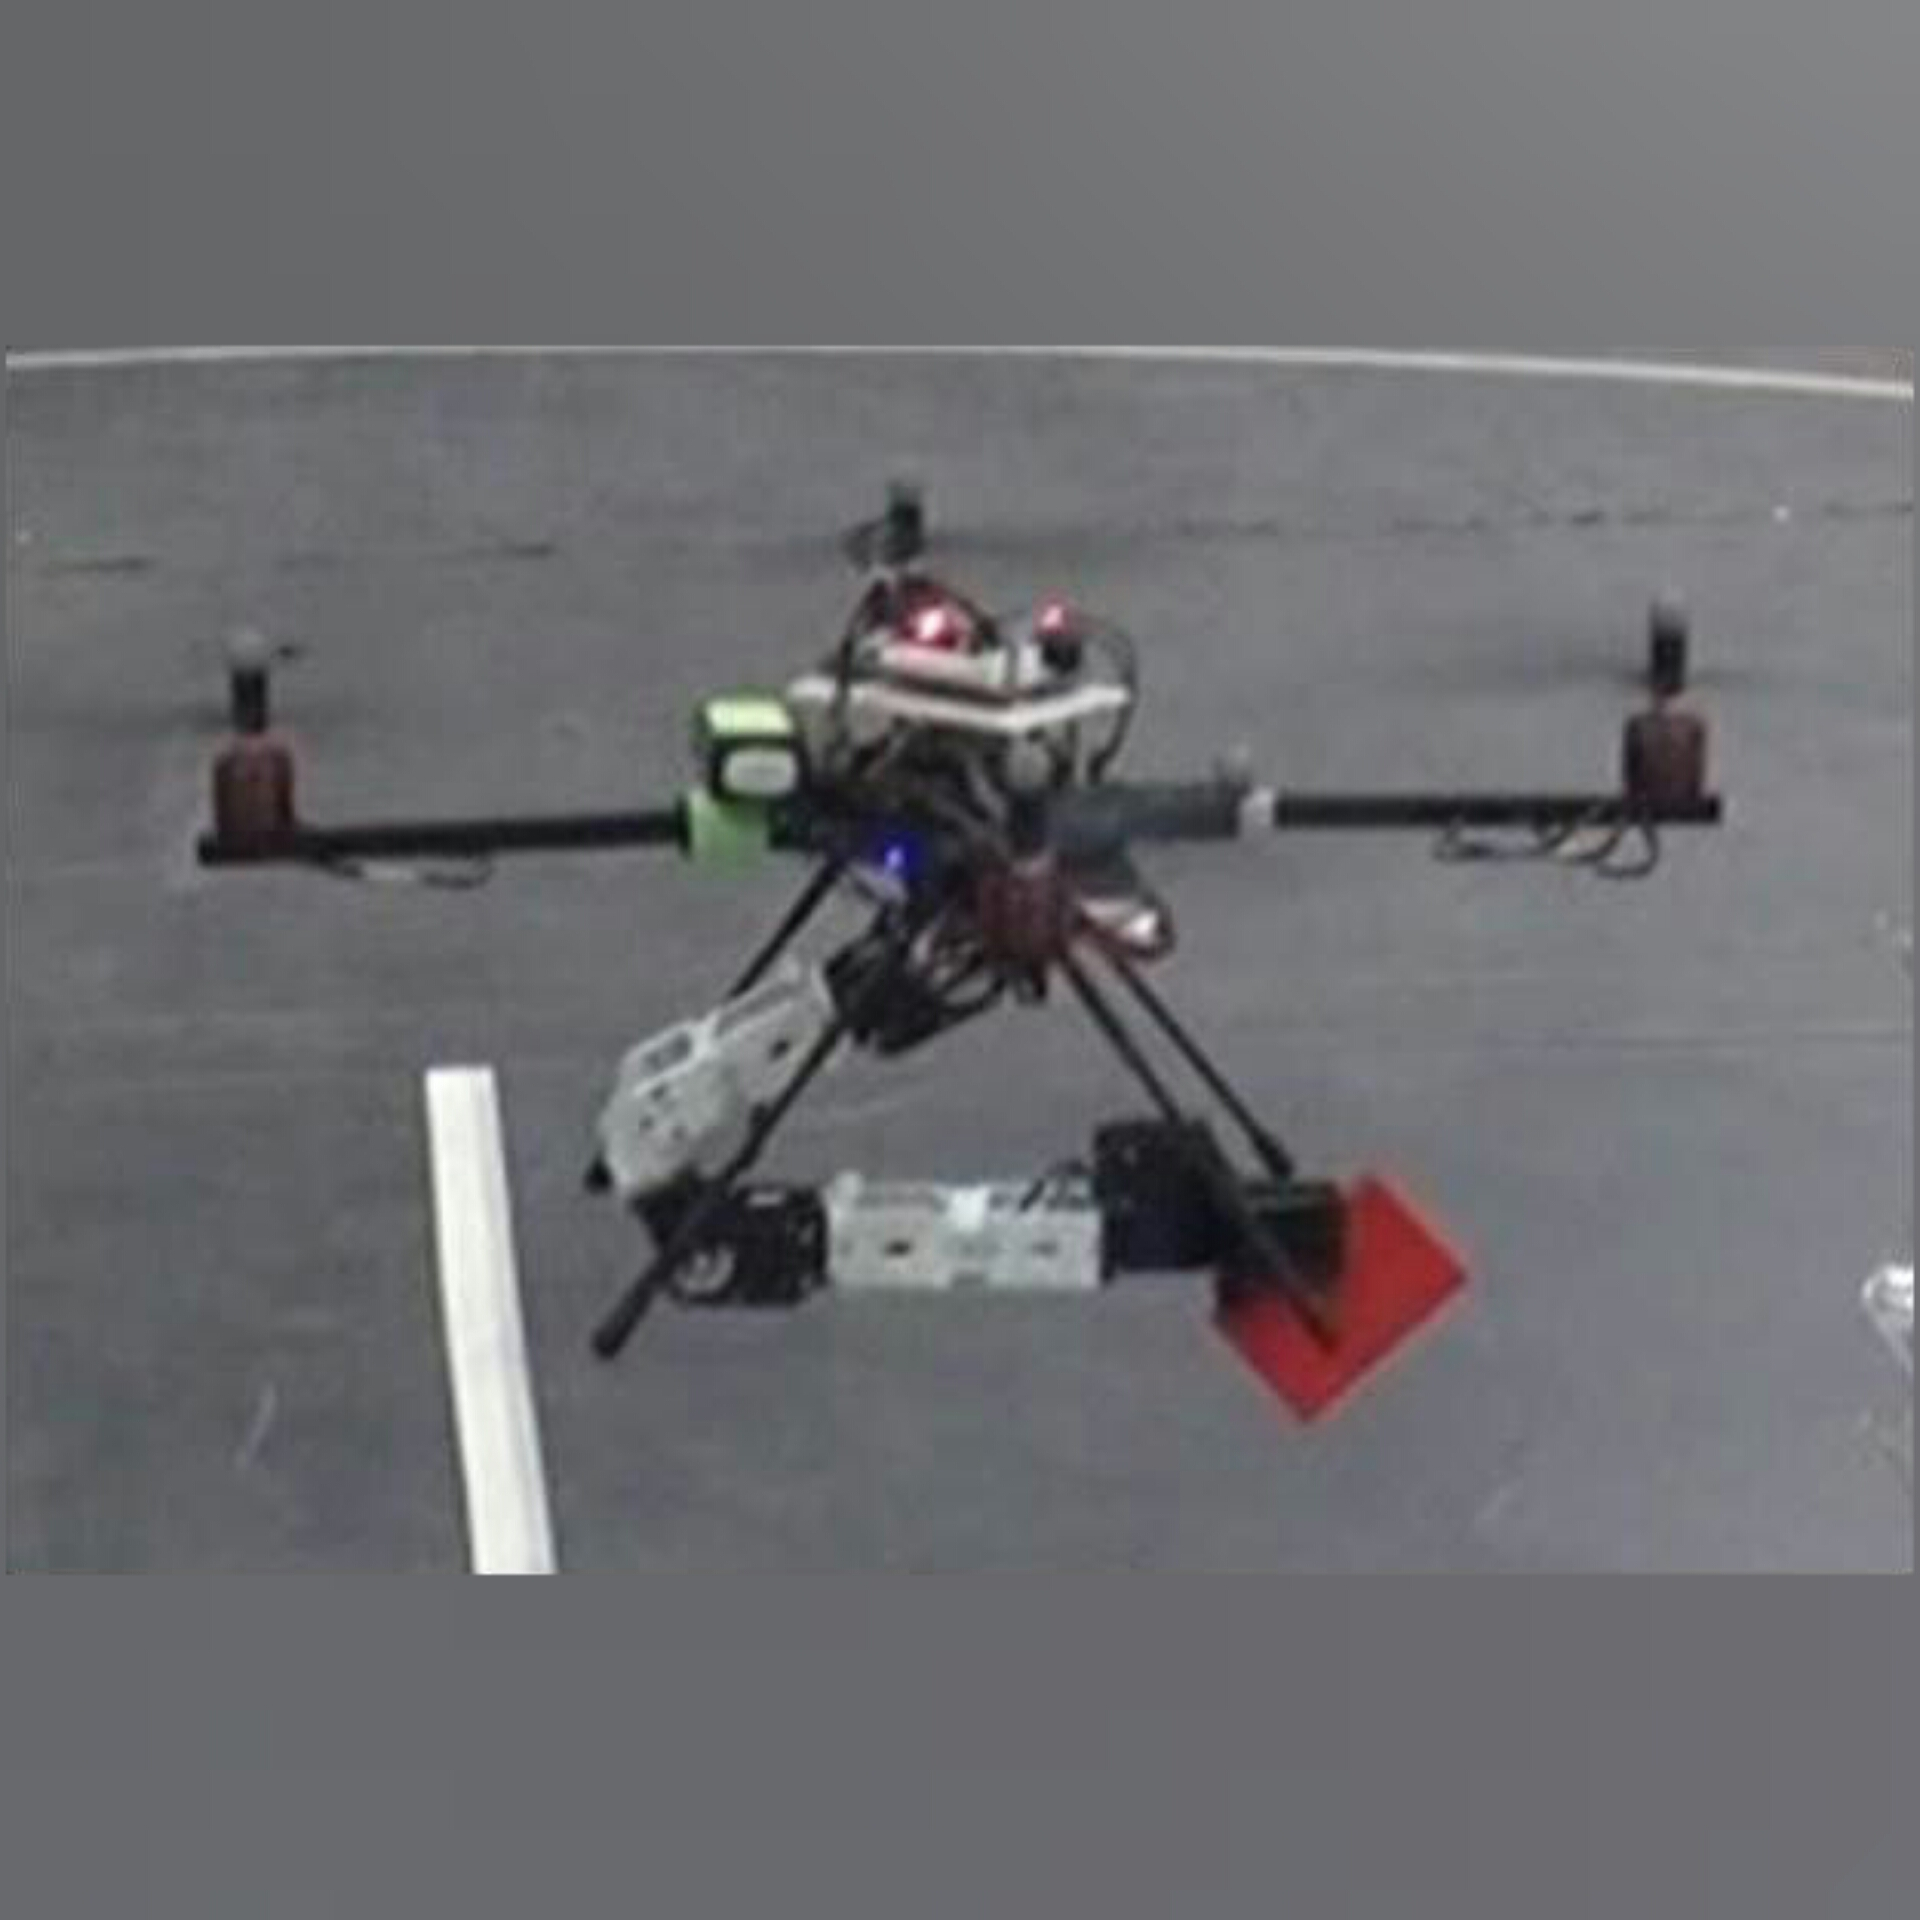
\includegraphics[width=0.6\textwidth]{imgs/kim.jpg}}
                    \caption*{\cite{Kim2013}}
                \end{figure}

            \end{column}
        \end{columns}
    }

    % subsection motiva_o (end)

    \subsection{Problema} % (fold)
    \label{sub:problema}

    \frame{
        \frametitle{Definição do Problema}

        \begin{columns}[c, onlytextwidth]
            \begin{column}[c]{0.6\textwidth}

                \justify
                Ambiente de trabalho conhecido e discretizado, possuindo os seguintes conjuntos:

                \begin{itemize}
                    \item Objetos a serem transportados;
                    \item Obstáculos;
                    \item Agentes disponíveis.
                \end{itemize}

                % \justify
                % Seja \workspace\ uma área de trabalho definida como $\workspace \subset \environment$, são definidos os conjuntos: \objectlist, possuindo os objetos a serem transportados, \obstaclelist, contendo obstáculos em \workspace\ e \robotlist, com todos os agentes disponíveis para a tarefa de transporte.
            \end{column}
            \begin{column}[c]{0.35\textwidth}
                \begin{figure}[p]
                    \centering
                    \setlength{\fboxsep}{0pt}
                    \fbox{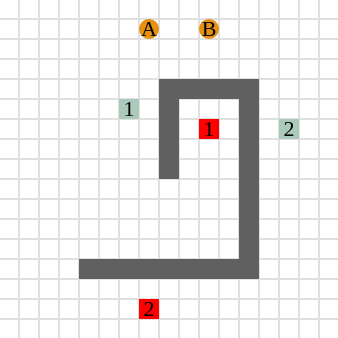
\includegraphics[width=0.95\textwidth]{imgs/example_1.png}}
                    \caption*{\centering Ambiente de Trabalho do Transporte}
                \end{figure}
            \end{column}
        \end{columns}
    }

    \frame{
        \frametitle{Definição do Problema}

        \begin{columns}[c, onlytextwidth]
            \begin{column}[c]{0.6\textwidth}
                \begin{block}{Problema 1}
                    \justify
                     Descrever uma sequência de poses válidas para os objetos que garantam a chegada dos mesmos às suas posições finais desejadas.
                \end{block}
            \end{column}
            \begin{column}[c]{0.35\textwidth}
                \begin{figure}[p]
                    \centering
                    \setlength{\fboxsep}{0pt}
                    \fbox{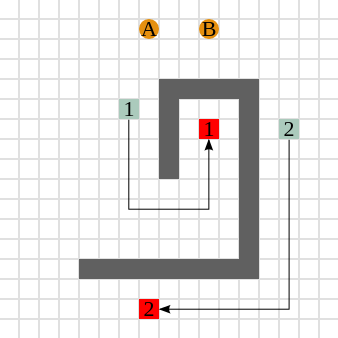
\includegraphics[width=0.95\textwidth]{imgs/example_2.png}}
                    \caption*{\centering Planejamento de caminho dos Objetos}
                \end{figure}
            \end{column}
        \end{columns}
    }

    \frame{
        \frametitle{Definição do Problema}

        \begin{columns}[c, onlytextwidth]
            \begin{column}[c]{0.6\textwidth}
                \begin{block}{Problema 2}
                    \justify
                    Tendo como base os planos de manipulação dos objetos, distribuir as tarefas entre os agentes disponíveis e coordená-los de modo a executarem o transporte dos objetos.
                \end{block}
            \end{column}
            \begin{column}[c]{0.35\textwidth}
                \begin{figure}[p]
                    \centering
                    \setlength{\fboxsep}{0pt}
                    \fbox{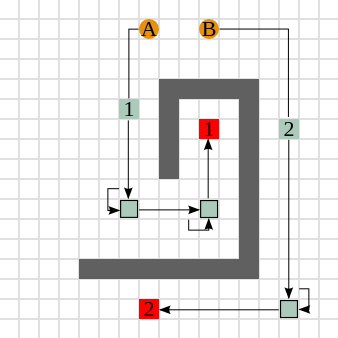
\includegraphics[width=0.95\textwidth]{imgs/example_3.png}}
                    \caption*{\centering Alocação de Tarefas e Execução}
                \end{figure}
            \end{column}
        \end{columns}
    }

    % subsection problema (end)
    % section introdu_o (end)

    \section{Trabalhos Relacionados} % (fold)
    \label{sec:trabalhos_relacionados}

    \frame{
        \frametitle{Trabalhos Relacionados}

        Alguns trabalhos que influenciaram o desenvolvimento da metodologia a ser apresentada compreendem as seguintes temáticas:

        \begin{itemize}
            \item Manipulação Não-preênsil;
            \item Manipulação Preênsil;
            \item Alocação de Tarefas e Coordenação de Agentes.
        \end{itemize}
    }

    \frame{
        \frametitle{Manipulação Não-preênsil}

        \begin{block}{Definição do Problema de \emph{box-pushing} (\cite{Mataric1995}):}
            \justify
            Seja um ambiente formado por itens rígidos, encontrar um caminho contínuo livre de obstáculos levando um objeto de sua posição inicial para outra posição final desejada utilizando somente ações de \emph{PUSH}. Demonstrado por \cite{Reif1979} ser \emph{NP-hard}.
        \end{block}
    }

    \frame{
        \frametitle{Manipulação Não-preênsil}

        \begin{columns}[c, onlytextwidth]
            \begin{column}[c]{0.5\textwidth}
                \begin{figure}[p]
                    \centering
                    \setlength{\fboxsep}{0pt}
                    \fbox{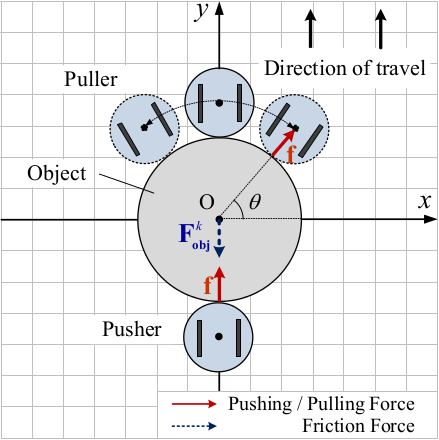
\includegraphics[width=0.95\textwidth]{imgs/libs/eoh_pp.png}}
                    \caption*{\centering \cite{Eoh2011}}
                \end{figure}
            \end{column}
            \begin{column}[c]{0.5\textwidth}
                \begin{figure}[p]
                    \centering
                    \setlength{\fboxsep}{0pt}
                    \fbox{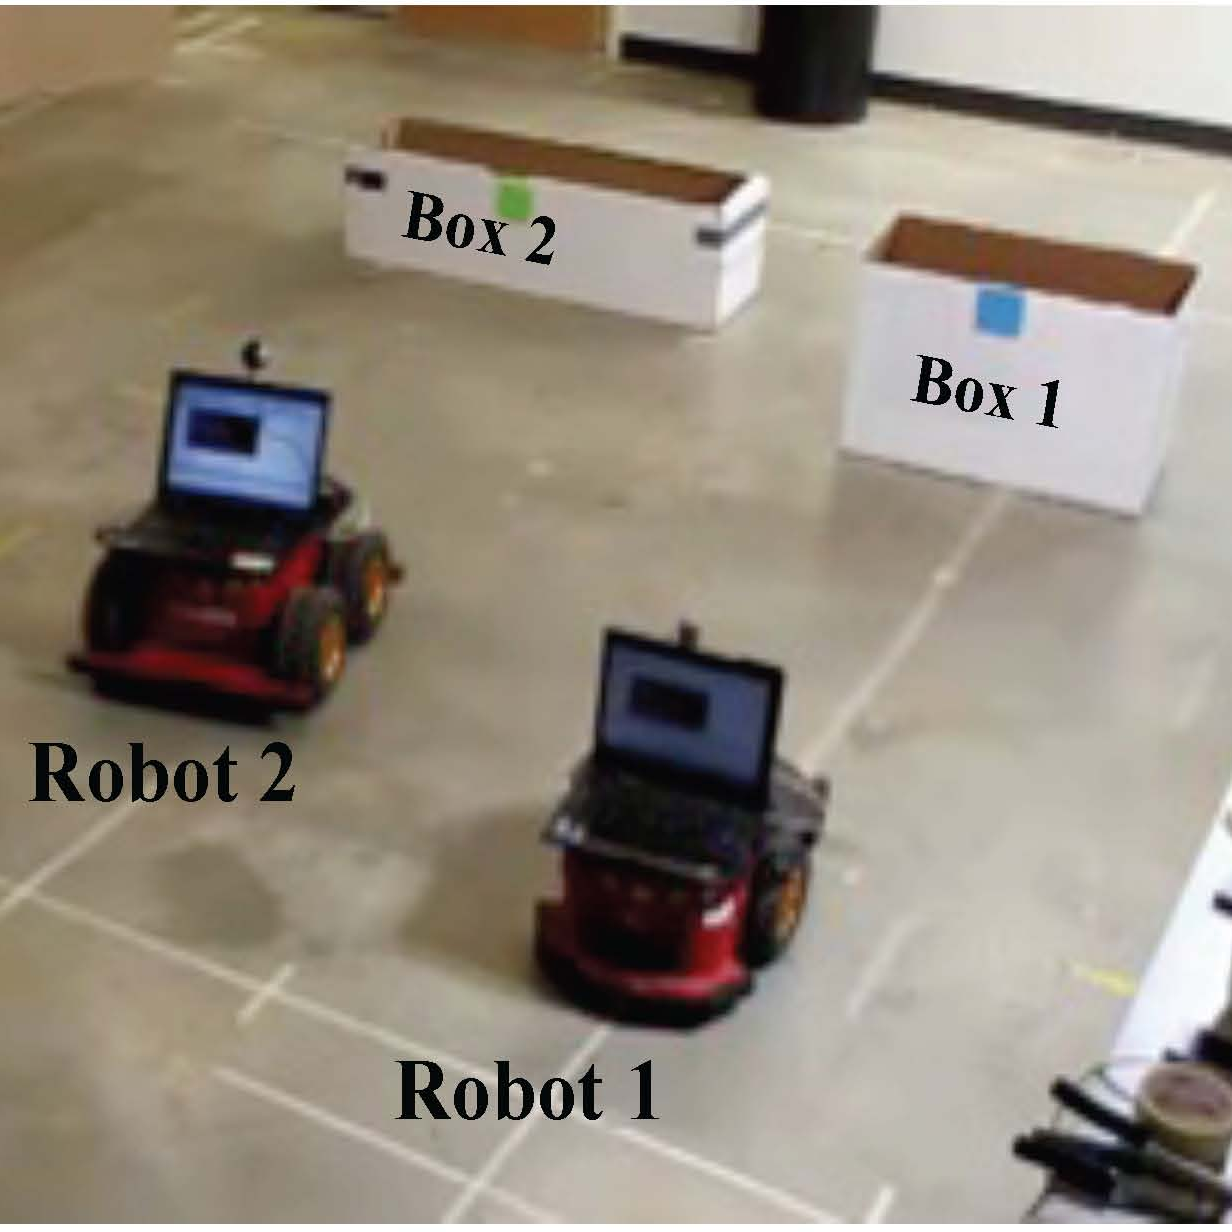
\includegraphics[width=0.95\textwidth]{imgs/libs/magh.png}}
                    \caption*{\centering \cite{Maghsoud2014}}
                \end{figure}
            \end{column}
        \end{columns}
    }

    \frame{
        \frametitle{Manipulação Não-preênsil}

        \begin{figure}[p]
            \centering
            \setlength{\fboxsep}{0pt}
            \fbox{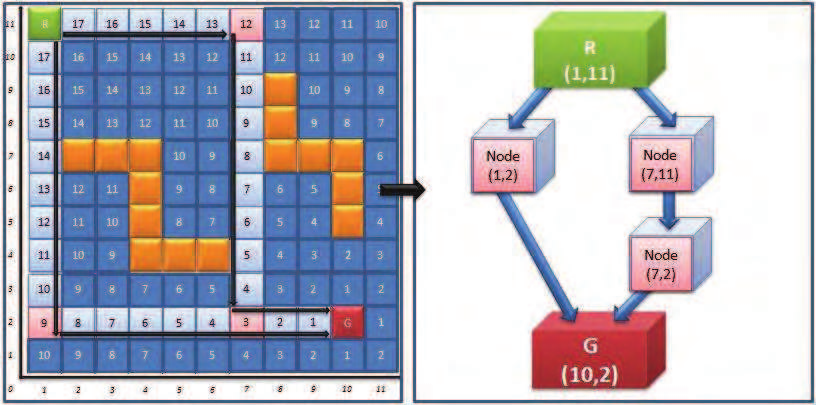
\includegraphics[width=0.9\textwidth]{imgs/libs/parra.png}}
            \caption*{\centering \cite{Parra-Gonzalez2012}}
        \end{figure}
    }

    % \frame{
        % OUT
        % \frametitle{Manipulação Preênsil}

        % \begin{figure}[p]
        %     \centering
        %     \setlength{\fboxsep}{0pt}
        %     \fbox{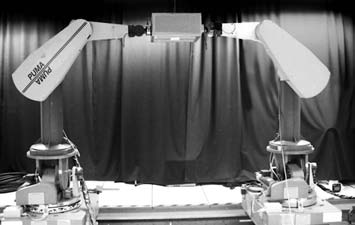
\includegraphics[width=0.7\textwidth]{imgs/libs/montemayor.png}}
        %     \caption*{\centering \cite{Montemayor2005}}
        % \end{figure}
    % }

    % \frame{
        % OUT
        % \frametitle{Manipulação Preênsil}

        % \begin{figure}[p]
        %     \centering
        %     \setlength{\fboxsep}{0pt}
        %     \fbox{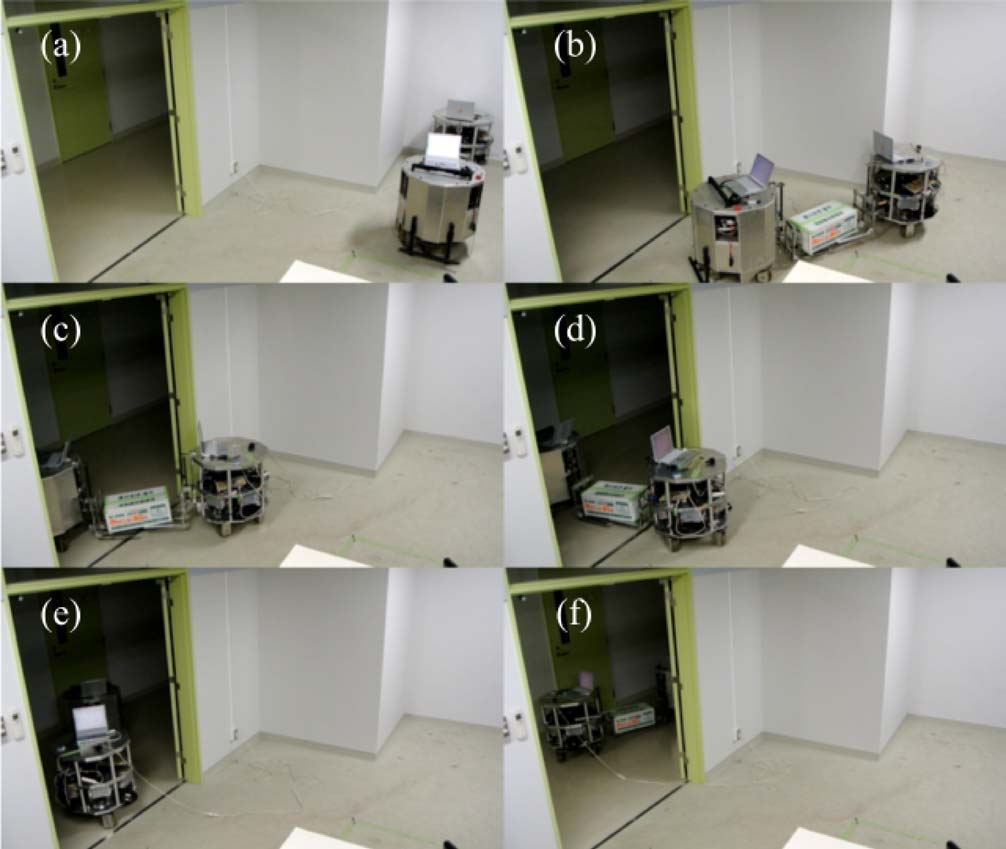
\includegraphics[width=0.6\textwidth]{imgs/libs/wada.png}}
        %     \caption*{\centering \cite{Wada2013}}
        % \end{figure}
    % }

    \frame{
        \frametitle{Manipulação Preênsil}

        \begin{columns}[c, onlytextwidth]
            \begin{column}[c]{0.5\textwidth}
                \begin{figure}[p]
                    \centering
                    \setlength{\fboxsep}{0pt}
                    \fbox{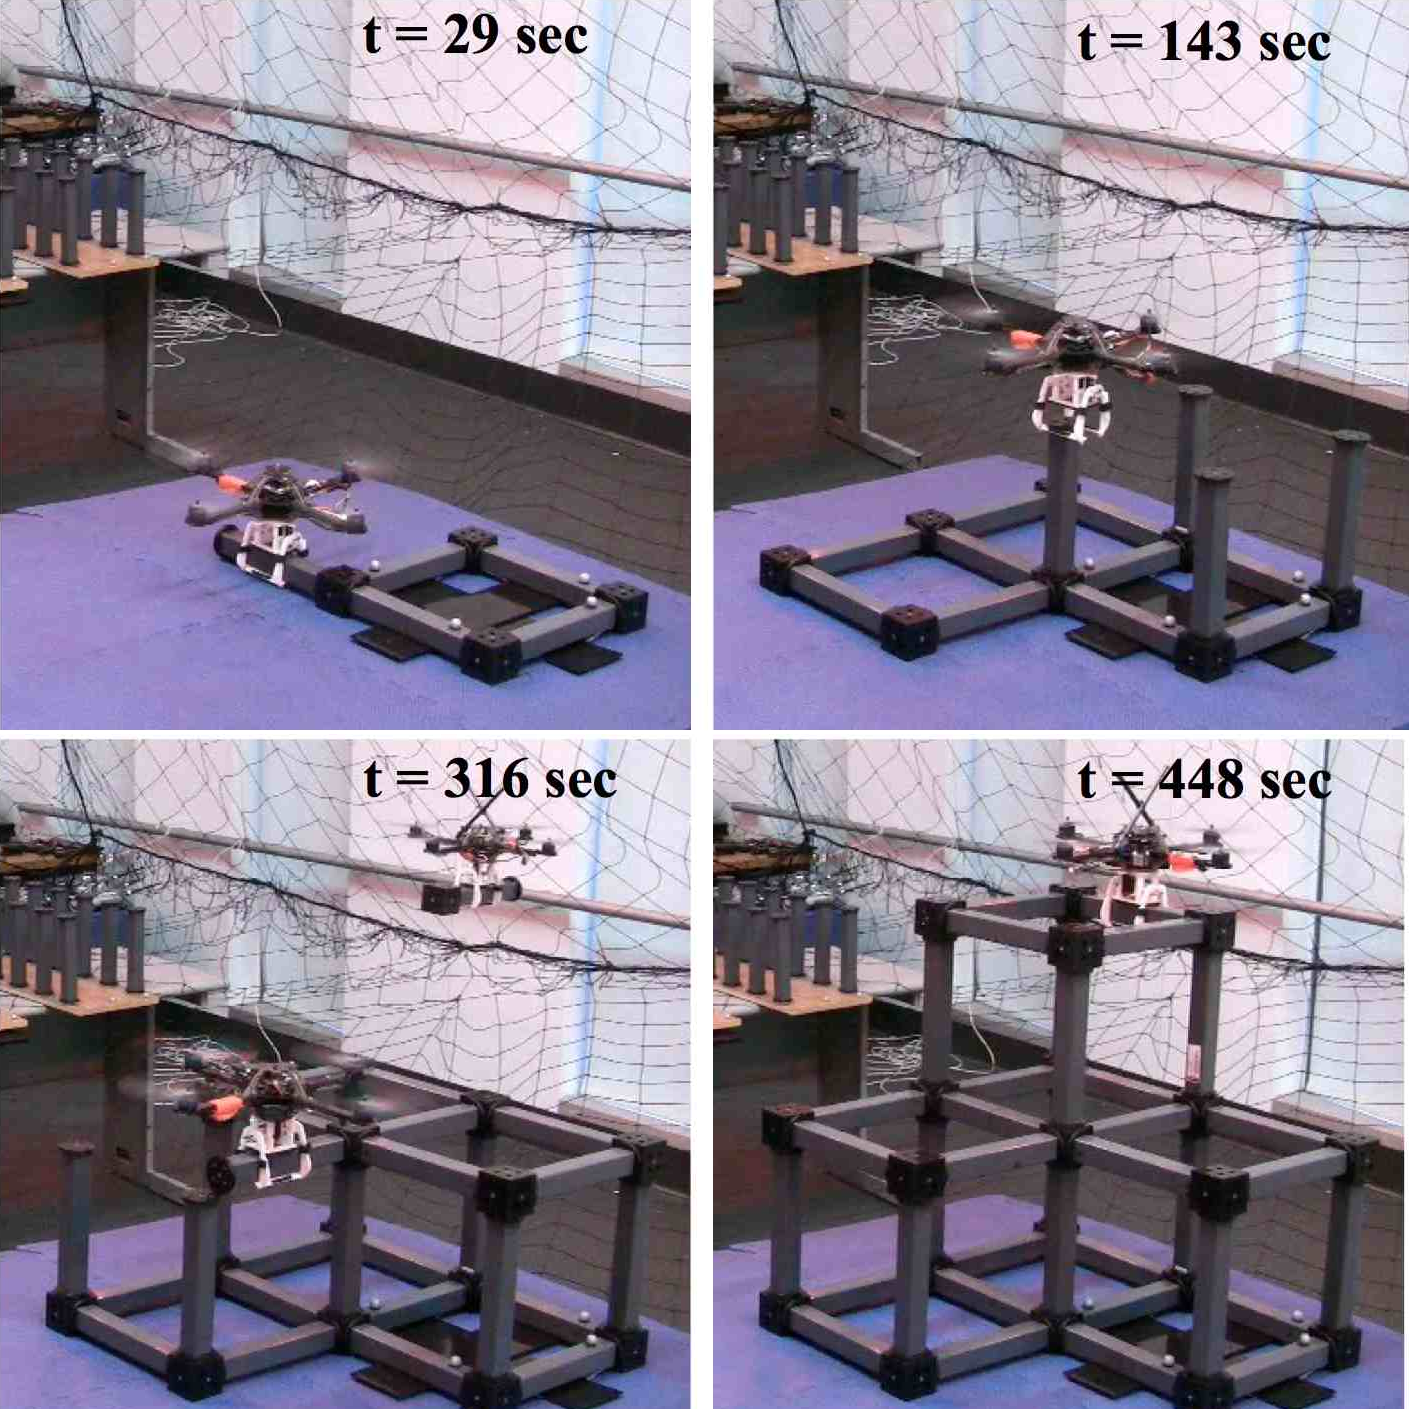
\includegraphics[width=0.95\textwidth]{imgs/libs/lindsey.png}}
                    \caption*{\centering \cite{Lindsey2012}}
                \end{figure}
            \end{column}
            \begin{column}[c]{0.5\textwidth}
                \begin{figure}[p]
                    \centering
                    \setlength{\fboxsep}{0pt}
                    \fbox{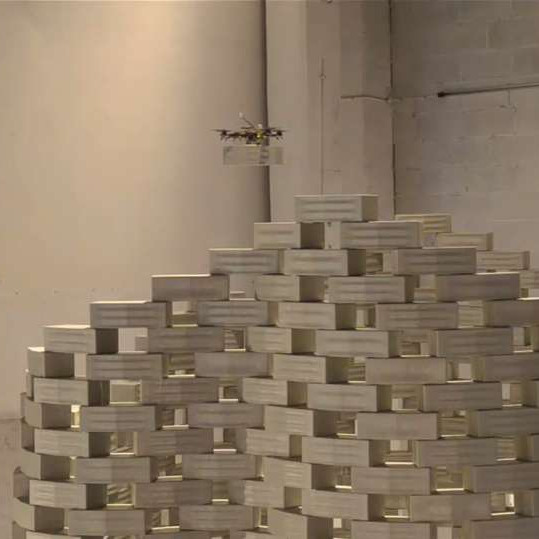
\includegraphics[width=0.95\textwidth]{imgs/libs/raffaello.jpg}}
                    \caption*{\centering \cite{Willmann2012}}
                \end{figure}
            \end{column}
        \end{columns}
    }

    \frame{
        \frametitle{Alocação de Tarefas}
        \begin{itemize}
            \item CoMutaR: A framework for multi-robot coordination and task allocation \cite{Shiroma2009};
            \item A fast and frugal method for team-task allocation in a multi-robot transportation system \cite{Wawerla2010};
            % \item A Multi-robot Exploration Approach Based on Distributed Graph Coloring \cite{Carvalho2013};
            \item Optimal bid valuation using path finding for multi-robot task allocation \cite{Oeztuerk2014}.
        \end{itemize}
    }

    % \frame{
    %     \frametitle{Alocação de Tarefas}
    % }

    % section trabalhos_relacionados (end)

    \section{Metodologia} % (fold)
    \label{sec:metodologia}

    \frame{
        \frametitle{Metodologia}

        \begin{figure}[p]
            \centering
            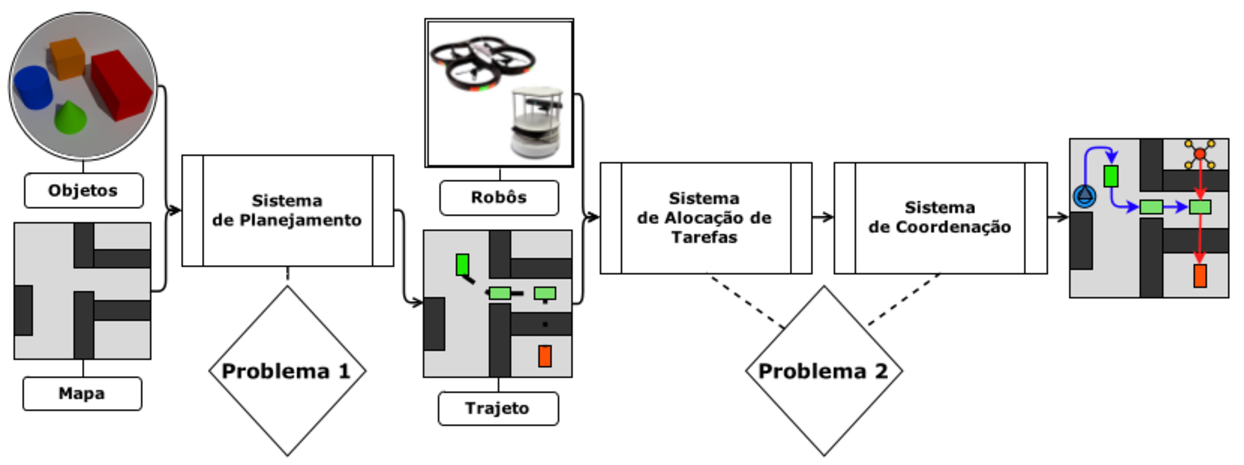
\includegraphics[width=\textwidth]{imgs/DiagramaGeral.pdf}
            \caption*{Diagrama Geral}
        \end{figure}
    }

    % \frame{
    %     \frametitle{Suposições}

    %     \begin{itemize}
    %         \item Localização de todos os itens no ambiente de trabalho é conhecida;
    %         \item Não existem no ambiente de trabalho demais corpos capazes de se mover além dos agentes;
    %         \item Existe um canal de comunicação entre os agentes, e o mesmo não possui falhas;
    %         \item Todos os objetos a serem transportados são iguais e de dimensões conhecidas.
    %     \end{itemize}
    % }

    \subsection{Definições}

    \frame{
        \frametitle{Ambiente de Trabalho}

        \begin{columns}[c, onlytextwidth]
            \begin{column}[c]{0.4\textwidth}
                % \begin{block}{Objetos}
                % \end{block}

                \begin{block}{Tipos de Agente}
                    \begin{itemize}
                        \item Terrestre: Ações \emph{PUSH};
                        \item Aéreo: Ações \emph{GRASP}.
                    \end{itemize}
                \end{block}

                % \justify
                % Agente que utiliza seu próprio corpo para aplicar a técnica de transporte não-preênsil (\emph{PUSH}), sem uso de manipuladores.
                % \begin{block}{Agente Aéreo}
                    % \justify
                    % Agente capaz de voar e faz uso de alguma técnica preênsil (\emph{GRASP}) para segurar o objeto e transportá-lo.
                % \end{block}
            \end{column}
            \begin{column}[c]{0.6\textwidth}
                \begin{figure}
                    \centering
                    \setlength{\fboxsep}{0pt}
                    \fbox{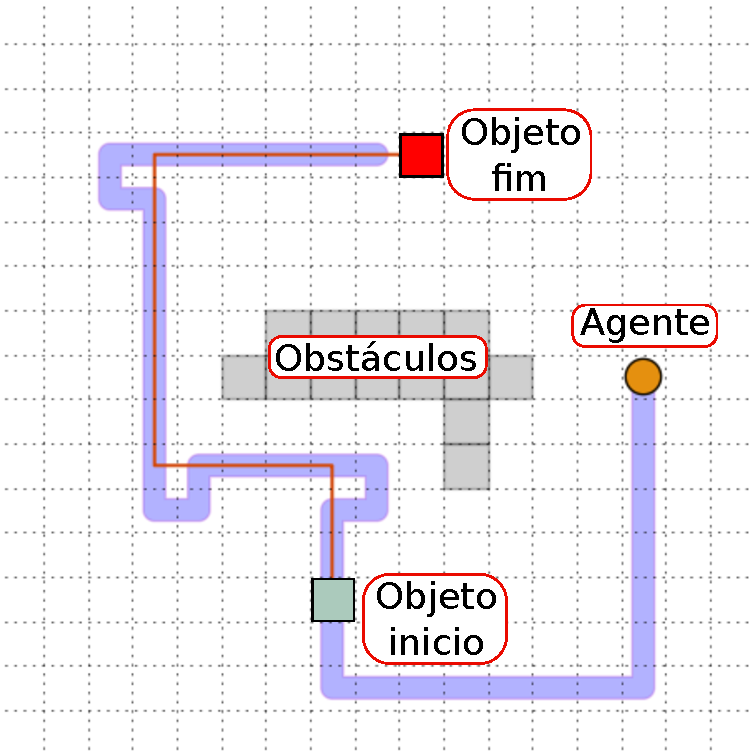
\includegraphics[width=0.9\textwidth]{imgs/mapa_exemplo.pdf}}
                \end{figure}
            \end{column}
        \end{columns}

    }

    % \frame{
        % OUT
        % \frametitle{Tipos de Agentes}

        % \begin{block}{Agente Terrestre}
        %     \justify
        %     Agente que utiliza seu próprio corpo para aplicar a técnica de transporte não-preênsil (\emph{PUSH}), sem uso de manipuladores.
        % \end{block}
        % \begin{columns}[c, onlytextwidth]
        %     \begin{column}[c]{0.8\textwidth}
        %     \end{column}
        %     \begin{column}[c]{0.2\textwidth}
        %         \begin{figure}[p]
        %             \centering
        %             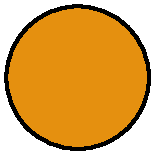
\includegraphics[width=0.5\textwidth]{imgs/robot_land.pdf}
        %         \end{figure}
        %     \end{column}
        % \end{columns}

        % \begin{block}{Agente Aéreo}
        %     \justify
        %     Agente capaz de voar e faz uso de alguma técnica preênsil (\emph{GRASP}) para segurar o objeto e transportá-lo.
        % \end{block}
        % \begin{columns}[c, onlytextwidth]
        %     \begin{column}[c]{0.8\textwidth}
        %     \end{column}
        %     \begin{column}[c]{0.2\textwidth}
        %         \begin{figure}[p]
        %             \centering
        %             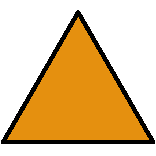
\includegraphics[width=0.5\textwidth]{imgs/robot_aerial.pdf}
        %         \end{figure}
        %     \end{column}
        % \end{columns}
    % }

    \frame{
        \frametitle{Função de Utilidade}

        \begin{block}{}
        \justify
        Quantifica a qualidade de um plano \planset\ considerando as dimensões: deslocamento (\timefunction) e energia (\energyfunction). Utilizada para comparar e selecionar os melhores planos para o transporte.
        \end{block}

        \begin{equation}
            \utilityfunction(\type{i}, \movementaction) = \alpha \cdot \timefunction(\type{i}, \movementaction) + (1 - \alpha) \cdot \energyfunction(\type{i}, \movementaction),
            \label{eq:util_function}
        \end{equation}

        \begin{equation}
          \utilityplanfunction(\planset) = \Big\{ \forall \plan{} \in \planset: \sum \utilityfunction(k(\plan{})) \Big\},
          \label{eq:plan_util_function}
        \end{equation}

        \begin{equation}
          k : \plan{} \mapsto \type{i}, \movementaction.
          \label{eq:get_data}
        \end{equation}

        % \begin{equation}
        %     <\alpha>\ =\{\alpha \in \mathbb{R} | 0 \leq \alpha \leq 1\}
        % \end{equation}

        \let\thefootnote\relax\footnotetext{\currentstate: estado atual, \type{i}: tipo do agente, \movementaction: ação}
    }

    \subsection{Planejamento de Caminhos -- Objeto}

    \frame{
        \frametitle{Planejamento de Caminhos -- Objeto}

        \begin{columns}[c]

            \begin{column}[c]{0.5\textwidth}
                \justify
                Planejamento para um objeto possui duas etapas:

                \begin{enumerate}
                    \item \emph{Planejamento}: no qual um plano de movimentação é criado;
                    \vspace{0.2cm}
                    \item \emph{Segmentação}: o plano gerado é segmentado em sub-planos.
                \end{enumerate}
            \end{column}

            \begin{column}[c]{0.5\textwidth}
                \begin{figure}[p]
                    \centering
                    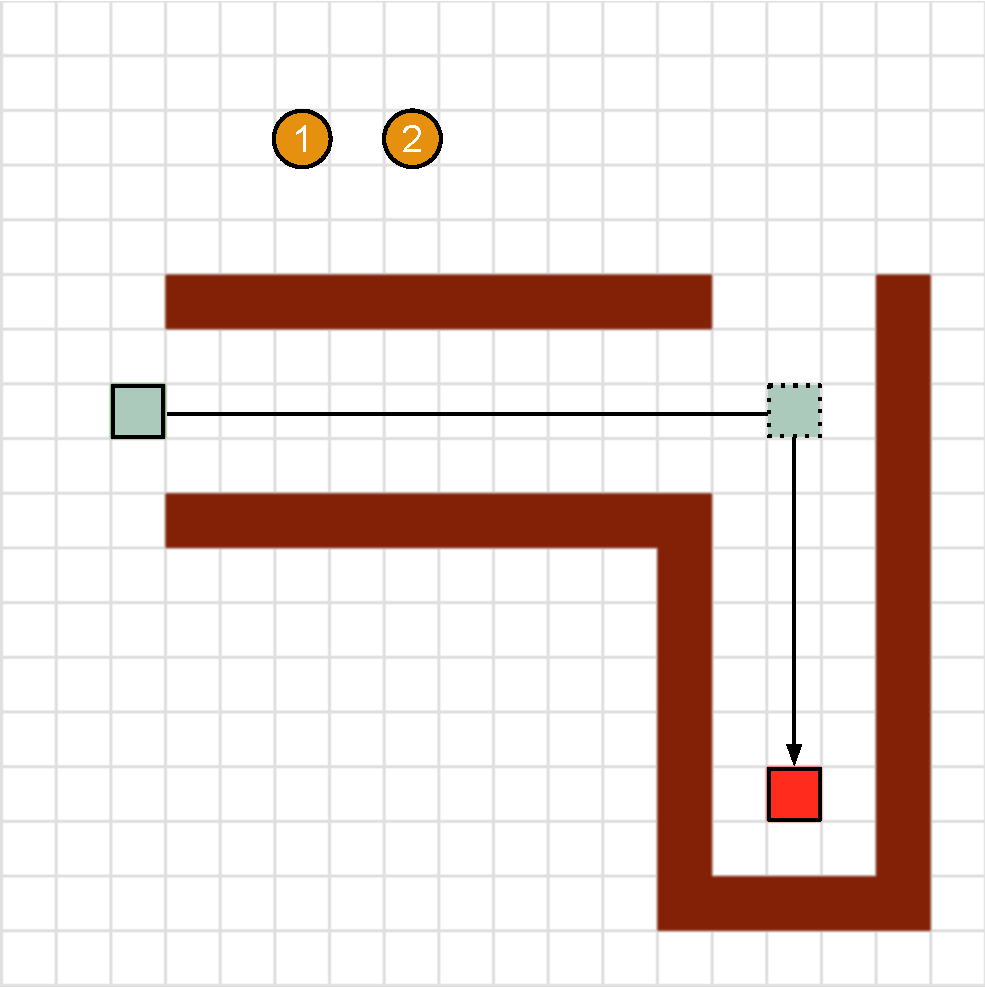
\includegraphics[width=0.9\textwidth]{imgs/ObjectMovement0.pdf}
                    \caption*{Plano para Objeto}
                \end{figure}
            \end{column}

        \end{columns}

        % \let\thefootnote\relax\footnotetext{\originstate: estado inicial, \targetstate: estado alvo}
    }

    \frame{
        \frametitle{Algoritmo de Planejamento}

        \begin{columns}[c]
            \begin{column}[c]{0.6\textwidth}
                \begin{block}{Baseado no Algoritmo A*}

                    Foram realizadas modificações nas seguintes etapas:

                    \begin{itemize}
                        \item Seleção do vértice para expansão;
                        \item Expansão da busca.
                    \end{itemize}

                \end{block}
            \end{column}
            \begin{column}[c]{0.4\textwidth}
                \fbox{\movie[height=0.9\textwidth, width=0.9\textwidth, autostart, loop]{}{astar.mp4}}
            \end{column}
        \end{columns}
    }

    \frame{
        \frametitle{Algoritmo de Planejamento -- Expansão da Busca}

        \begin{figure}[p]
            \setlength{\fboxsep}{0pt}
            \centering
            \begin{subfigure}[b]{0.32\textwidth}
                \fbox{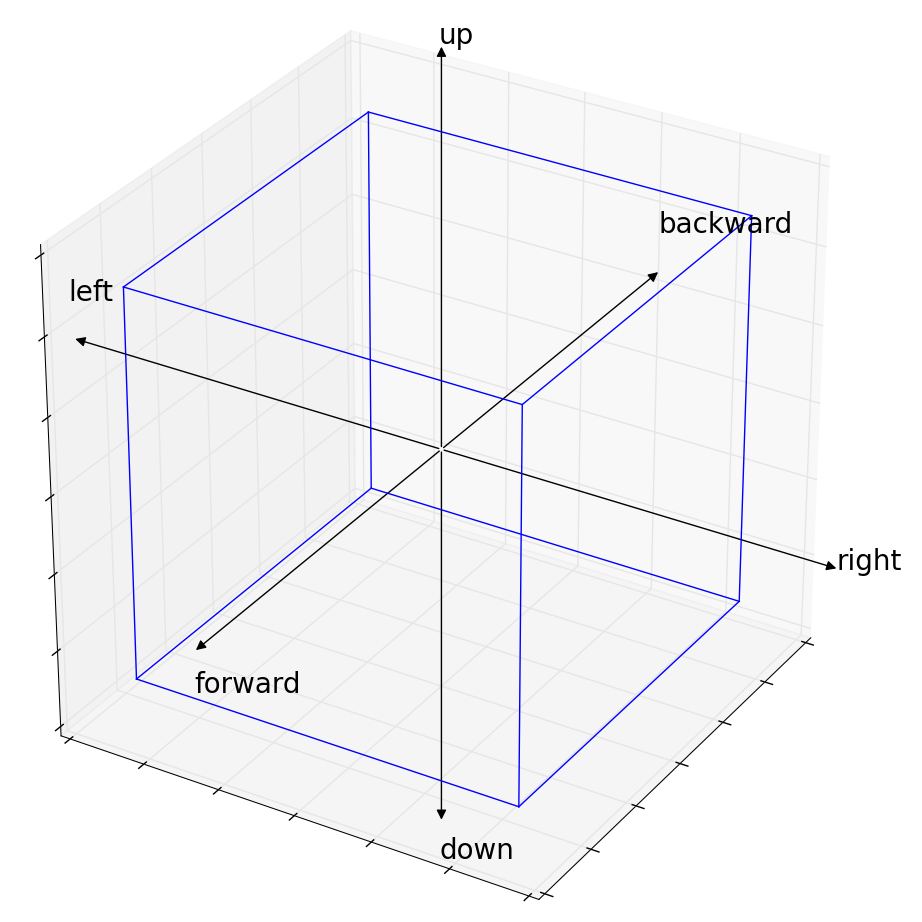
\includegraphics[width=\textwidth]{imgs/moves.png}}
                \caption*{Tipos de movimento}
            \end{subfigure}
            \begin{subfigure}[b]{0.32\textwidth}
                \fbox{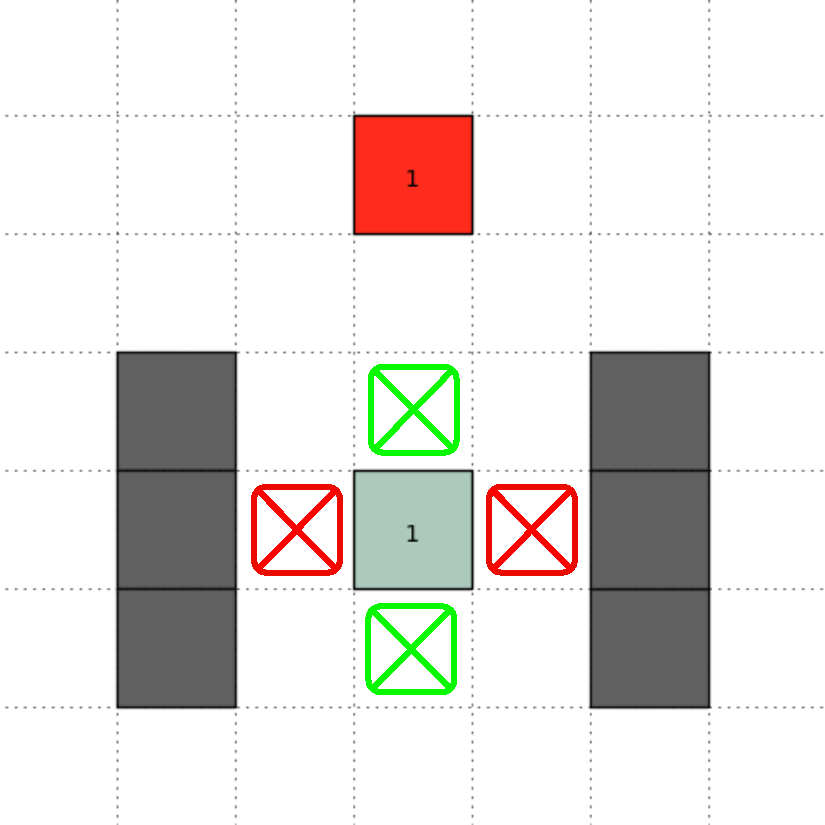
\includegraphics[width=\textwidth]{imgs/teste1.pdf}}
                \caption*{Validação do Movimento}
            \end{subfigure}
            \begin{subfigure}[b]{0.32\textwidth}
                \fbox{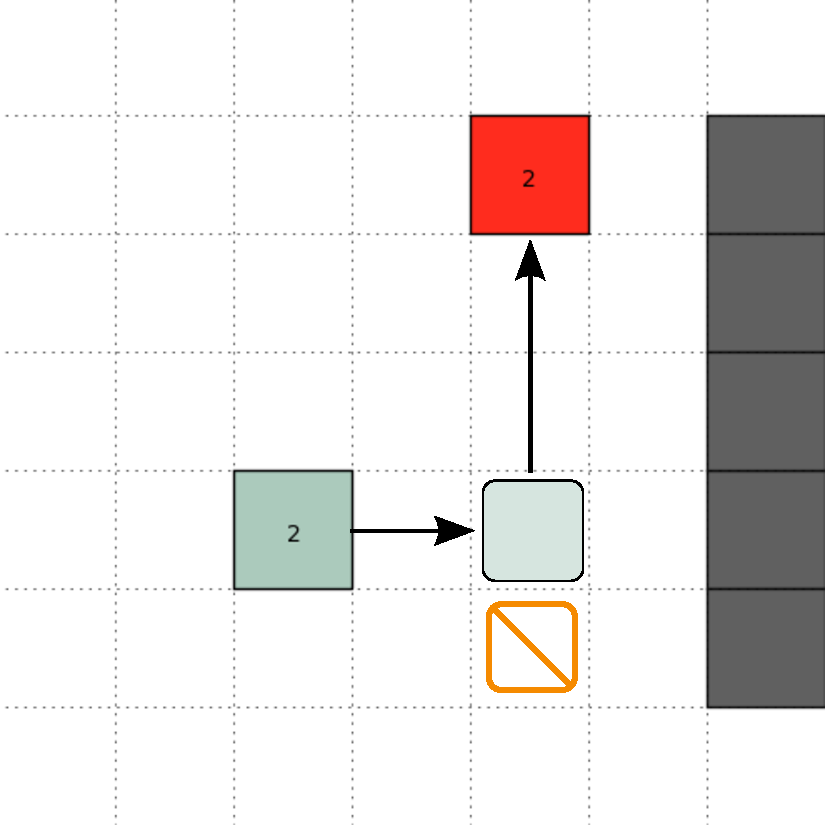
\includegraphics[width=\textwidth]{imgs/teste2.pdf}}
                \caption*{Penalização}
            \end{subfigure}
        \end{figure}
    }

    \frame{
        \frametitle{Algoritmo de Segmentação do Plano}

        \begin{columns}[c]

            \begin{column}[c]{0.5\textwidth}
                Segmentação ocorre em duas etapas:

                \begin{enumerate}
                    \item Criação dos pontos de segmentação;
                    \item Criação dos segmentos.
                \end{enumerate}
            \end{column}

            \begin{column}[c]{0.5\textwidth}
                \begin{figure}[p]
                    \centering
                    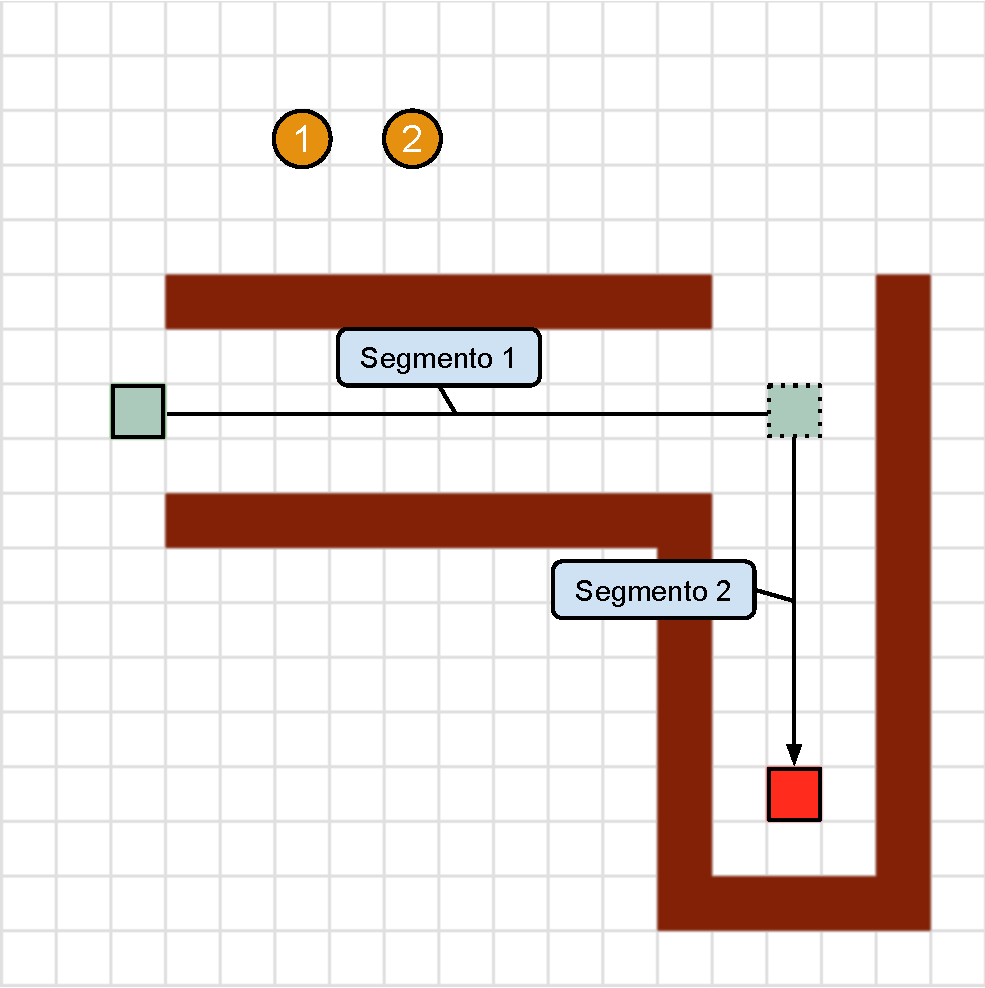
\includegraphics[width=0.9\textwidth]{imgs/ObjectMovement1.pdf}
                    \caption*{Segmentos do plano}
                \end{figure}
            \end{column}

        \end{columns}
    }

    \subsection{Planejamento de Caminhos -- Agentes}

    \frame{
        \frametitle{Planejamento de Caminhos - Agentes}

        \begin{columns}[c]
            \begin{column}[c]{0.5\textwidth}
                \justify
                Com base nos segmentos criados para o plano do objeto, para cada agente \robot{i}, são criados planos de movimentação de dois tipos:

                \begin{itemize}
                    \item \emph{Preparação}: plano no qual o agente se aproxima do objeto a ser transportado;
                    \vspace{0.2cm}
                    \item \emph{Transporte}: plano que realiza a movimentação do objeto.
                \end{itemize}

                Esta etapa ocorre durante a Alocação de Tarefas.

            \end{column}
            \begin{column}[c]{0.5\textwidth}
                \begin{figure}[p]
                    \centering
                    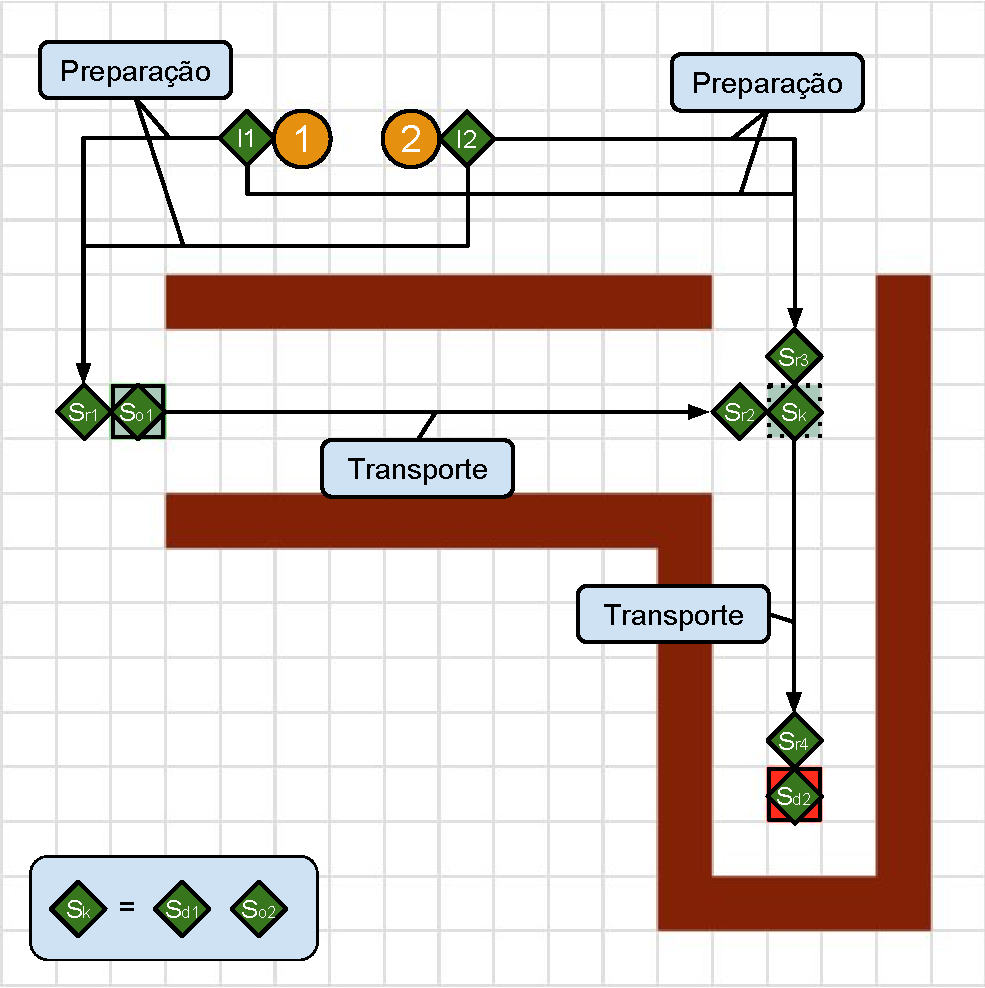
\includegraphics[width=0.9\textwidth]{imgs/ObjectMovement2.pdf}
                    \caption*{Plano para os Agentes}
                \end{figure}
            \end{column}
        \end{columns}
    }

    \subsection{Alocação de Tarefas}

    \frame{
        \frametitle{Alocação de Tarefas}

        \begin{figure}[p]
            \centering
            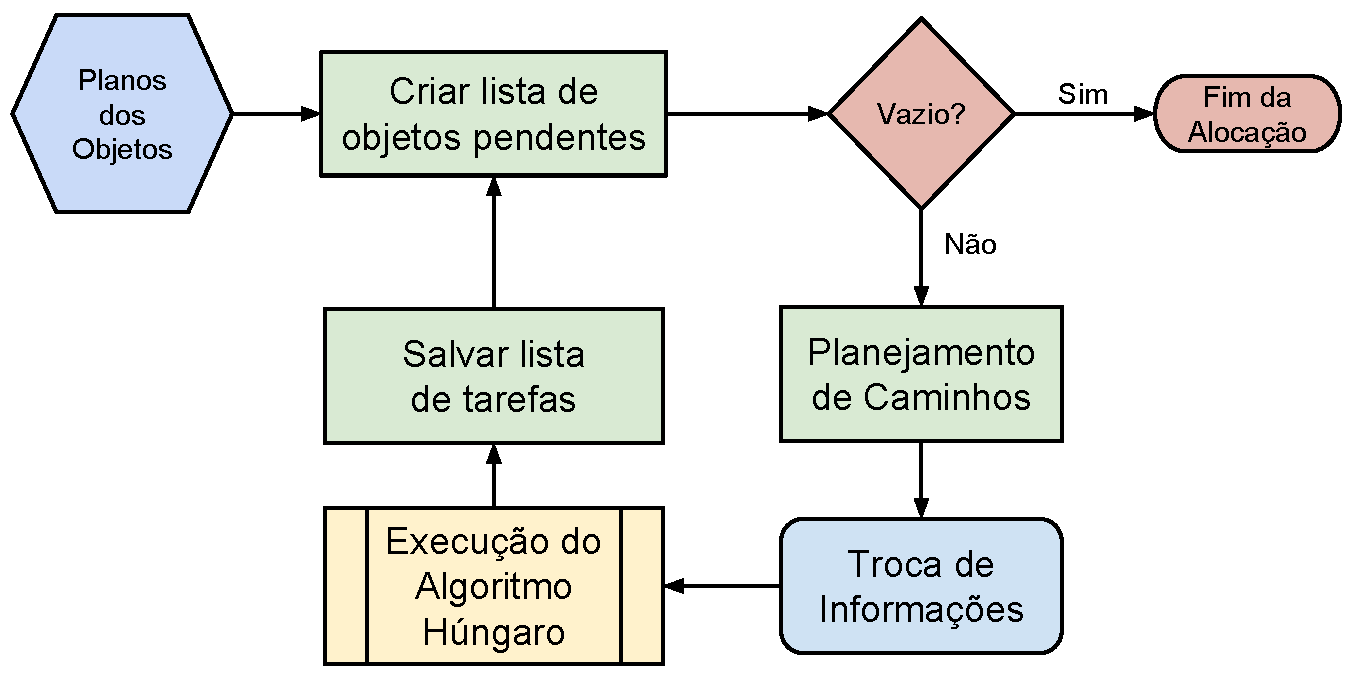
\includegraphics[width=0.95\textwidth]{imgs/TaskAllocationProcess.pdf}
        \end{figure}

        % \begin{enumerate}
        %     \item Criar lista de objetos pendentes;
        %     \item Planejamento dos planos de transporte para cada agente;
        %     \item Troca de informações entre os agentes;
        %     \item Alocação dos planos usando o Algoritmo Húngaro;
        %     \item Cada agente atualiza a própria lista de tarefas;
        %     \item Repetir até todos os objetos serem alocados.
        % \end{enumerate}
    }

    % \frame{
    %     \frametitle{Alocação de Tarefas -- Algoritmo Húngaro}
    % }

    \subsection{Coordenação e Execução} % (fold)

    % \frame{
    %     \frametitle{Coordenação e Execução}
    %     Coordenação entre os agentes é inspirada na técnica de redes de computadores \emph{Token Ring}, realizada mediante a troca de \emph{tokens}.

    %     \begin{figure}[p]
    %         \centering
    %         \setlength{\fboxsep}{0pt}
    %         \fbox{\movie[height=0.3\textwidth, width=0.6615\textwidth, autostart, loop]{}{tokenring.mp4}}
    %     \end{figure}
    % }

    \frame{
        \frametitle{Coordenação e Execução}

        \begin{block}{}
        \justify
        Coordenação mediante a troca de \emph{token}, baseado em uma técnica de redes de computadores. Cada objeto possui dois tipos de \emph{token}:
        \end{block}

        % Coordenação entre os agentes é inspirada na técnica de redes de computadores \emph{Token Ring}, realizada mediante a troca de \emph{tokens}.
        % Para cada objeto existem dois tipos de \emph{token}, seguindo as regras:

        \vspace{0.3cm}

        \begin{enumerate}
            \item Para cada segmento, são criados \emph{tokens} do tipo $<$preparação$>$;
            \item É criado um \emph{token} do tipo $<$transporte$>$.
        \end{enumerate}

        \vspace{0.3cm}

        \begin{block}{}
        \justify
        Baseado nesta técnica, o objeto é transportado por um único agente em cada segmento, os demais agentes podem realizar o passo de preparação ou transportar outros objetos.
        \end{block}

        % Desta maneira, somente um agente é capaz de transportar o objeto, enquanto os demais podem realizar o passo de preparação.
        % Uma vez o segmento de transporte seja completado, o \emph{token} deste pode ser disponibilizado a outro agente.
    }

    \subsection{Exemplo} % (fold)

    \frame{
        \frametitle{Exemplo de Transporte}

        \centering
        \movie[height=0.55\textwidth, width=0.614\textwidth, autostart, loop]{}{execution.mp4}

        % \begin{columns}[c]
        %     \begin{column}[c]{0.5\textwidth}
        %         \begin{figure}[p]
        %             \centering
        %             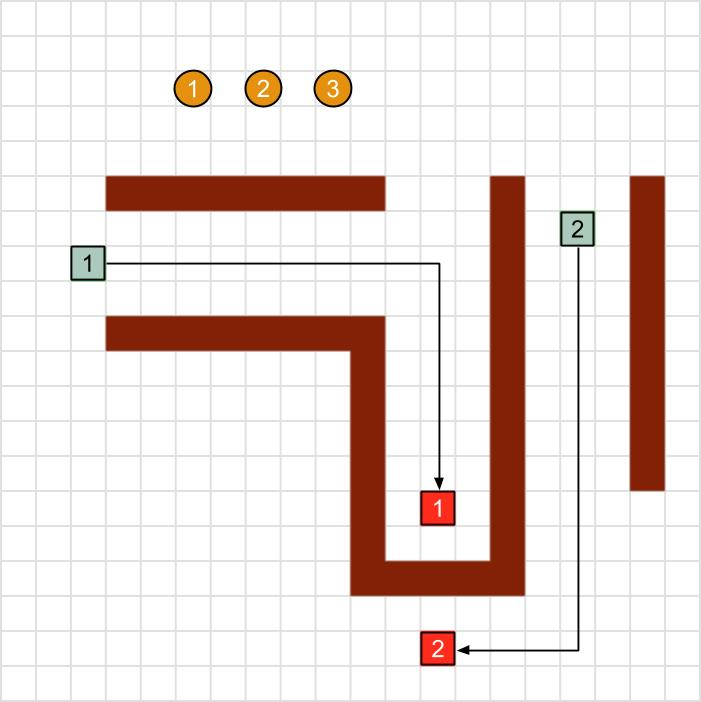
\includegraphics[width=0.9\textwidth]{imgs/execution/Mov1.jpg}
        %             \caption*{Planejamento dos Objetos}
        %         \end{figure}
        %     \end{column}
        %     \begin{column}[c]{0.5\textwidth}
        %         \begin{figure}[p]
        %             \centering
        %             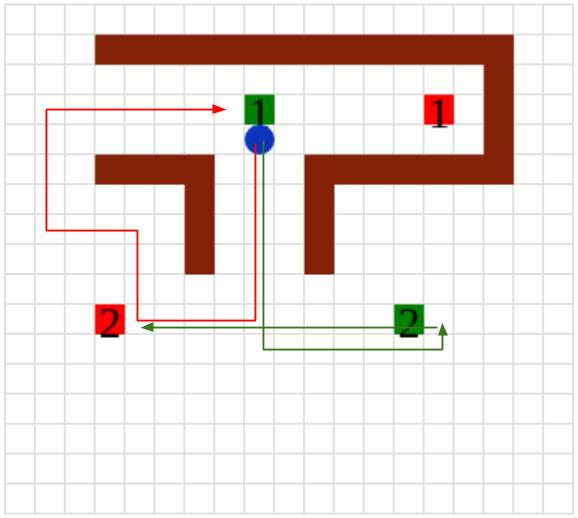
\includegraphics[width=0.9\textwidth]{imgs/execution/Mov2.jpg}
        %             \caption*{Primeira Alocação}
        %         \end{figure}
        %     \end{column}
        % \end{columns}
    }

    % \frame{
        % OUT
        % \frametitle{Exemplo de Transporte}

        % \begin{columns}[c]
        %     \begin{column}[c]{0.5\textwidth}
        %         \begin{figure}[p]
        %             \centering
        %             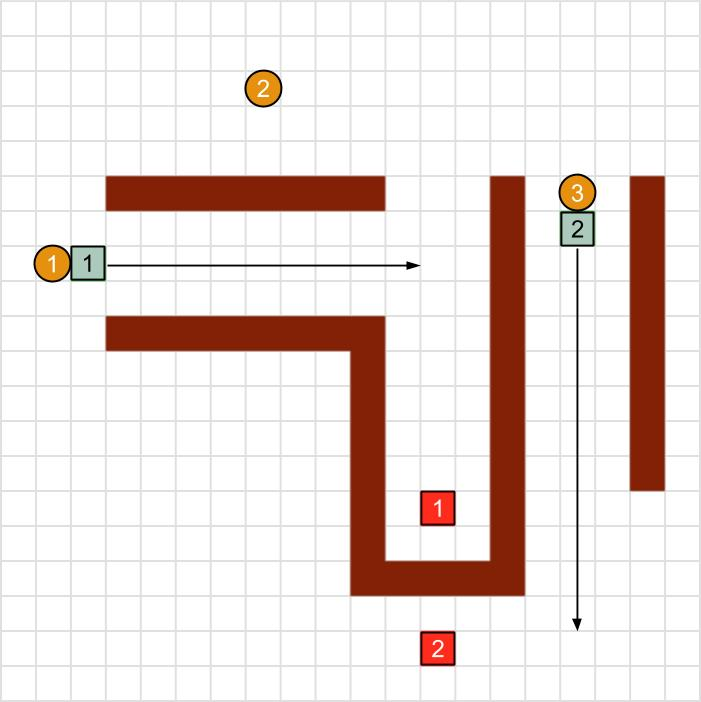
\includegraphics[width=0.9\textwidth]{imgs/execution/Mov3.jpg}
        %             \caption*{Execução do transporte}
        %         \end{figure}
        %     \end{column}
        %     \begin{column}[c]{0.5\textwidth}
        %         \begin{figure}[p]
        %             \centering
        %             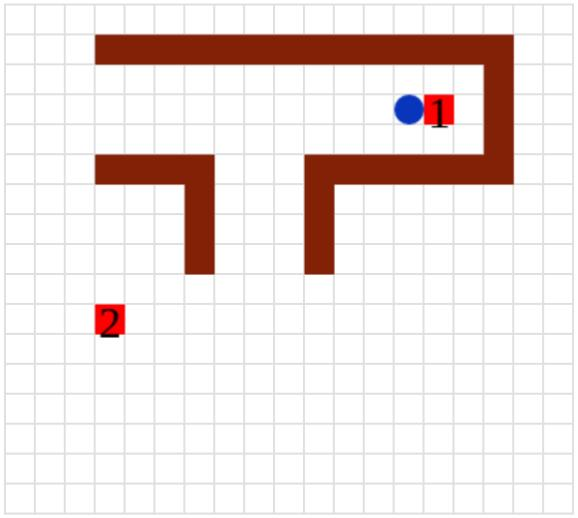
\includegraphics[width=0.9\textwidth]{imgs/execution/Mov4.jpg}
        %             \caption*{Segunda Alocação}
        %         \end{figure}
        %     \end{column}
        % \end{columns}
    % }

    % \frame{
        % OUT
        % \frametitle{Exemplo de Transporte}

        % \begin{columns}[c]
        %     \begin{column}[c]{0.5\textwidth}
        %         \begin{figure}[p]
        %             \centering
        %             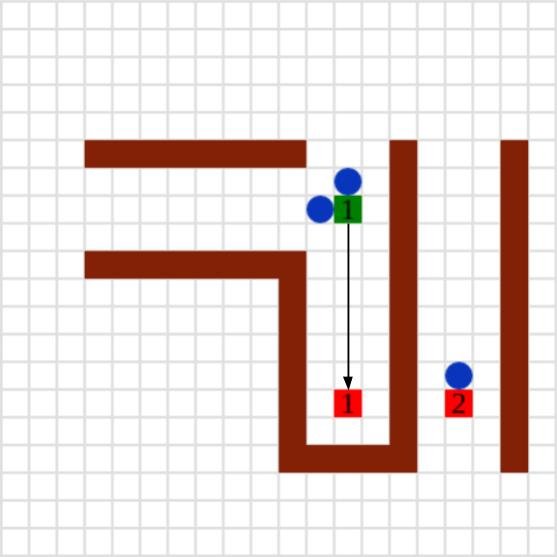
\includegraphics[width=0.9\textwidth]{imgs/execution/Mov5.jpg}
        %             \caption*{Execução do transporte}
        %         \end{figure}
        %     \end{column}
        %     \begin{column}[c]{0.5\textwidth}
        %         \begin{figure}[p]
        %             \centering
        %             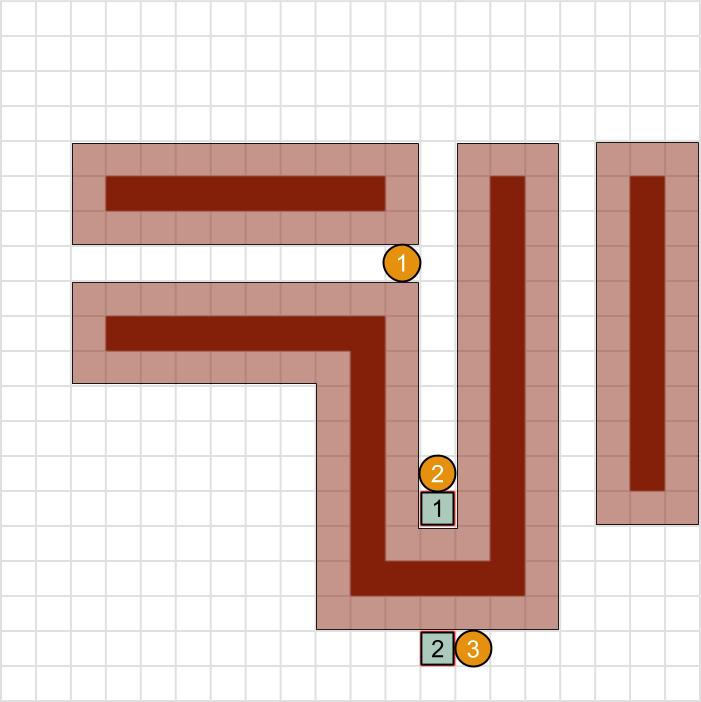
\includegraphics[width=0.9\textwidth]{imgs/execution/Mov6.jpg}
        %             \caption*{Finalização do Transporte}
        %         \end{figure}
        %     \end{column}
        % \end{columns}
    % }

    % section metodologia (end)

    \section{Experimentos} % (fold)
    \label{sec:experimentos}

    \frame{
        \frametitle{Experimentos}

        \begin{figure}[p]
            \centering
            \setlength{\fboxsep}{0pt}
            \begin{subfigure}[b]{0.32\textwidth}
                \centering
                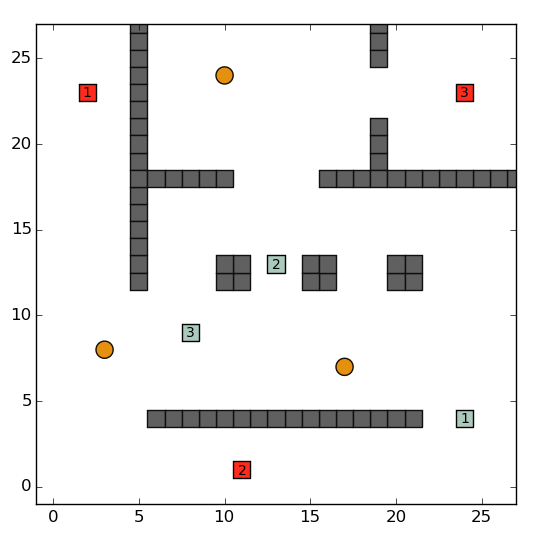
\includegraphics[width=0.7\textwidth]{imgs/experimentos/ambient_4.png}
                \caption*{\centering Complexidade}
            \end{subfigure}
            \begin{subfigure}[b]{0.32\textwidth}
                \centering
                \fbox{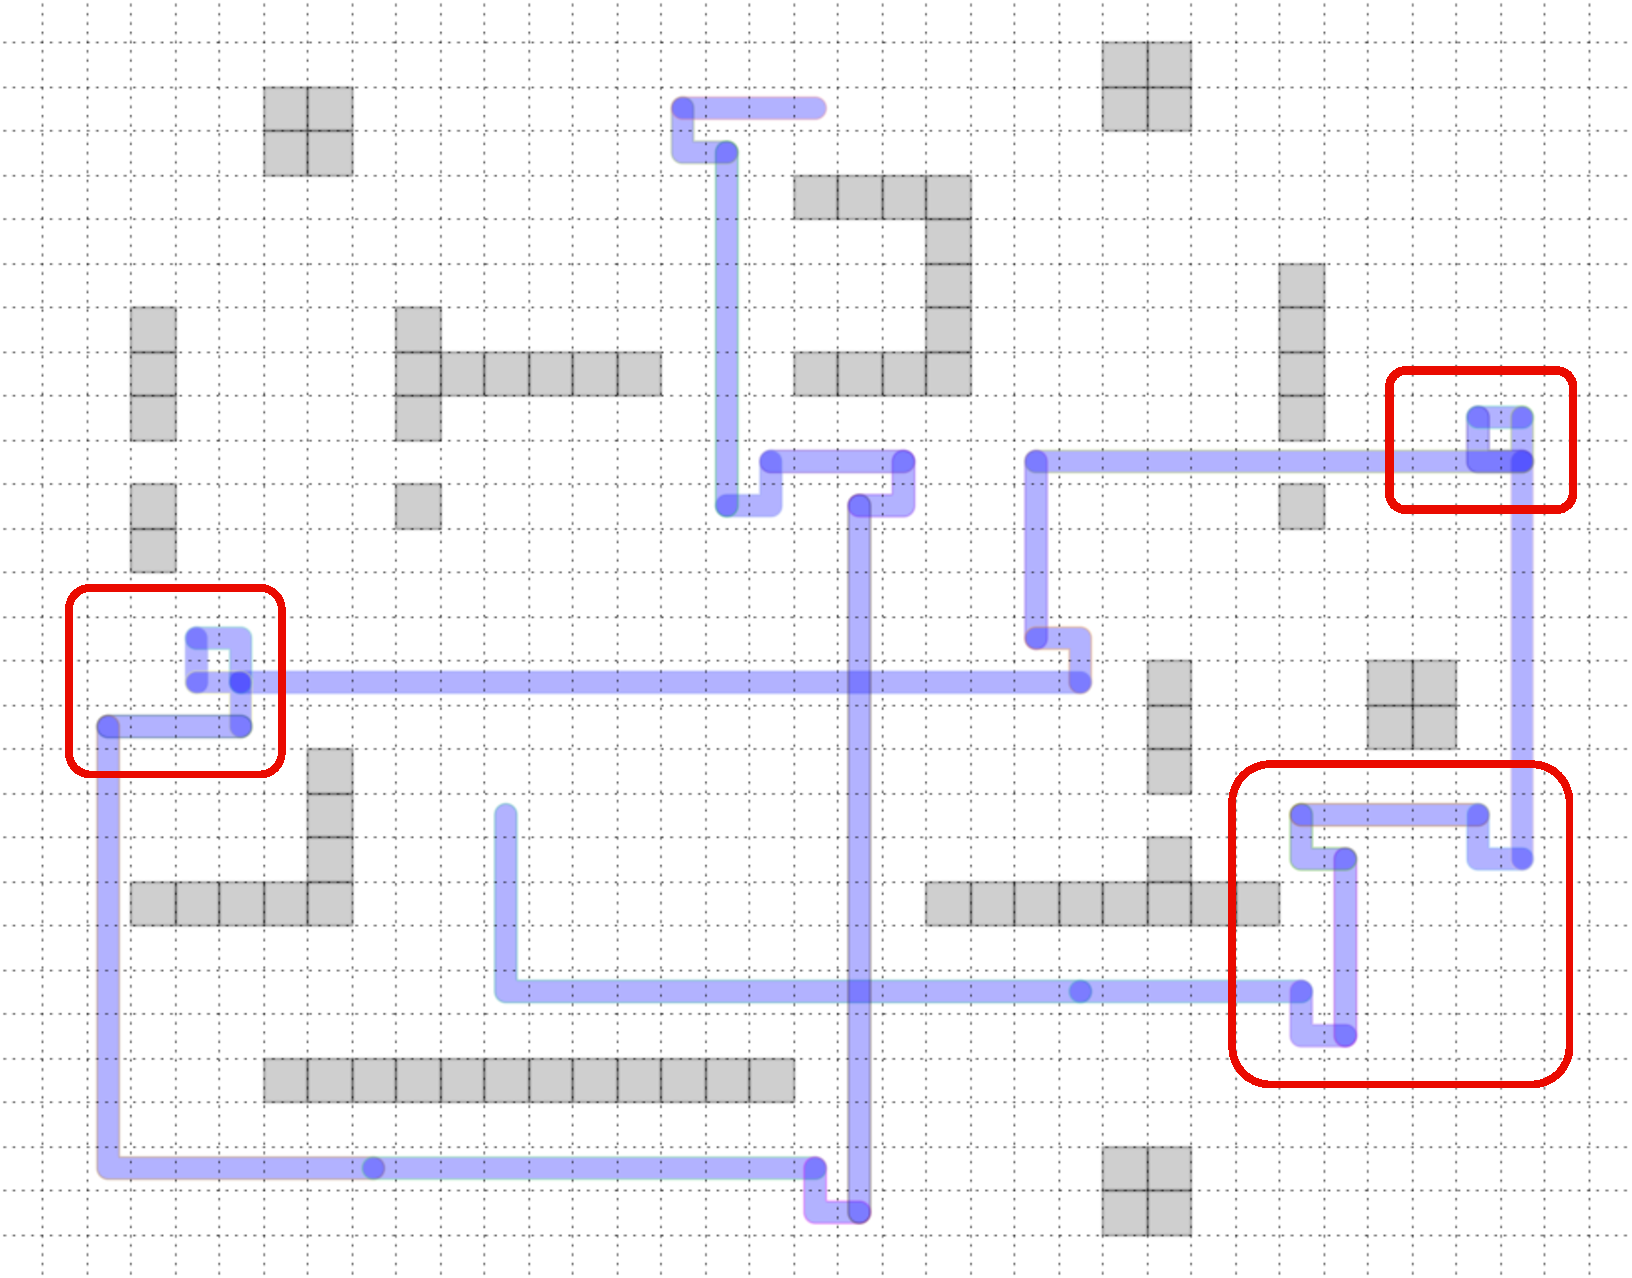
\includegraphics[width=0.7\textwidth, height=0.7\textwidth]{imgs/experimentos/ambiente_penalizacao_sem.pdf}}
                \caption*{\centering Penalização}
            \end{subfigure}
            \begin{subfigure}[b]{0.32\textwidth}
                \centering
                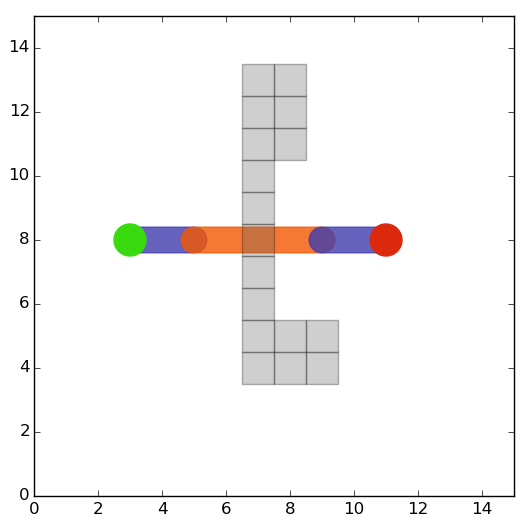
\includegraphics[width=0.7\textwidth]{imgs/experimentos/utility_func_mid.png}
                \caption*{\centering Função de Utilidade}
            \end{subfigure}\\
            \vspace{0.1cm}
            \begin{subfigure}[b]{0.32\textwidth}
                \centering
                \fbox{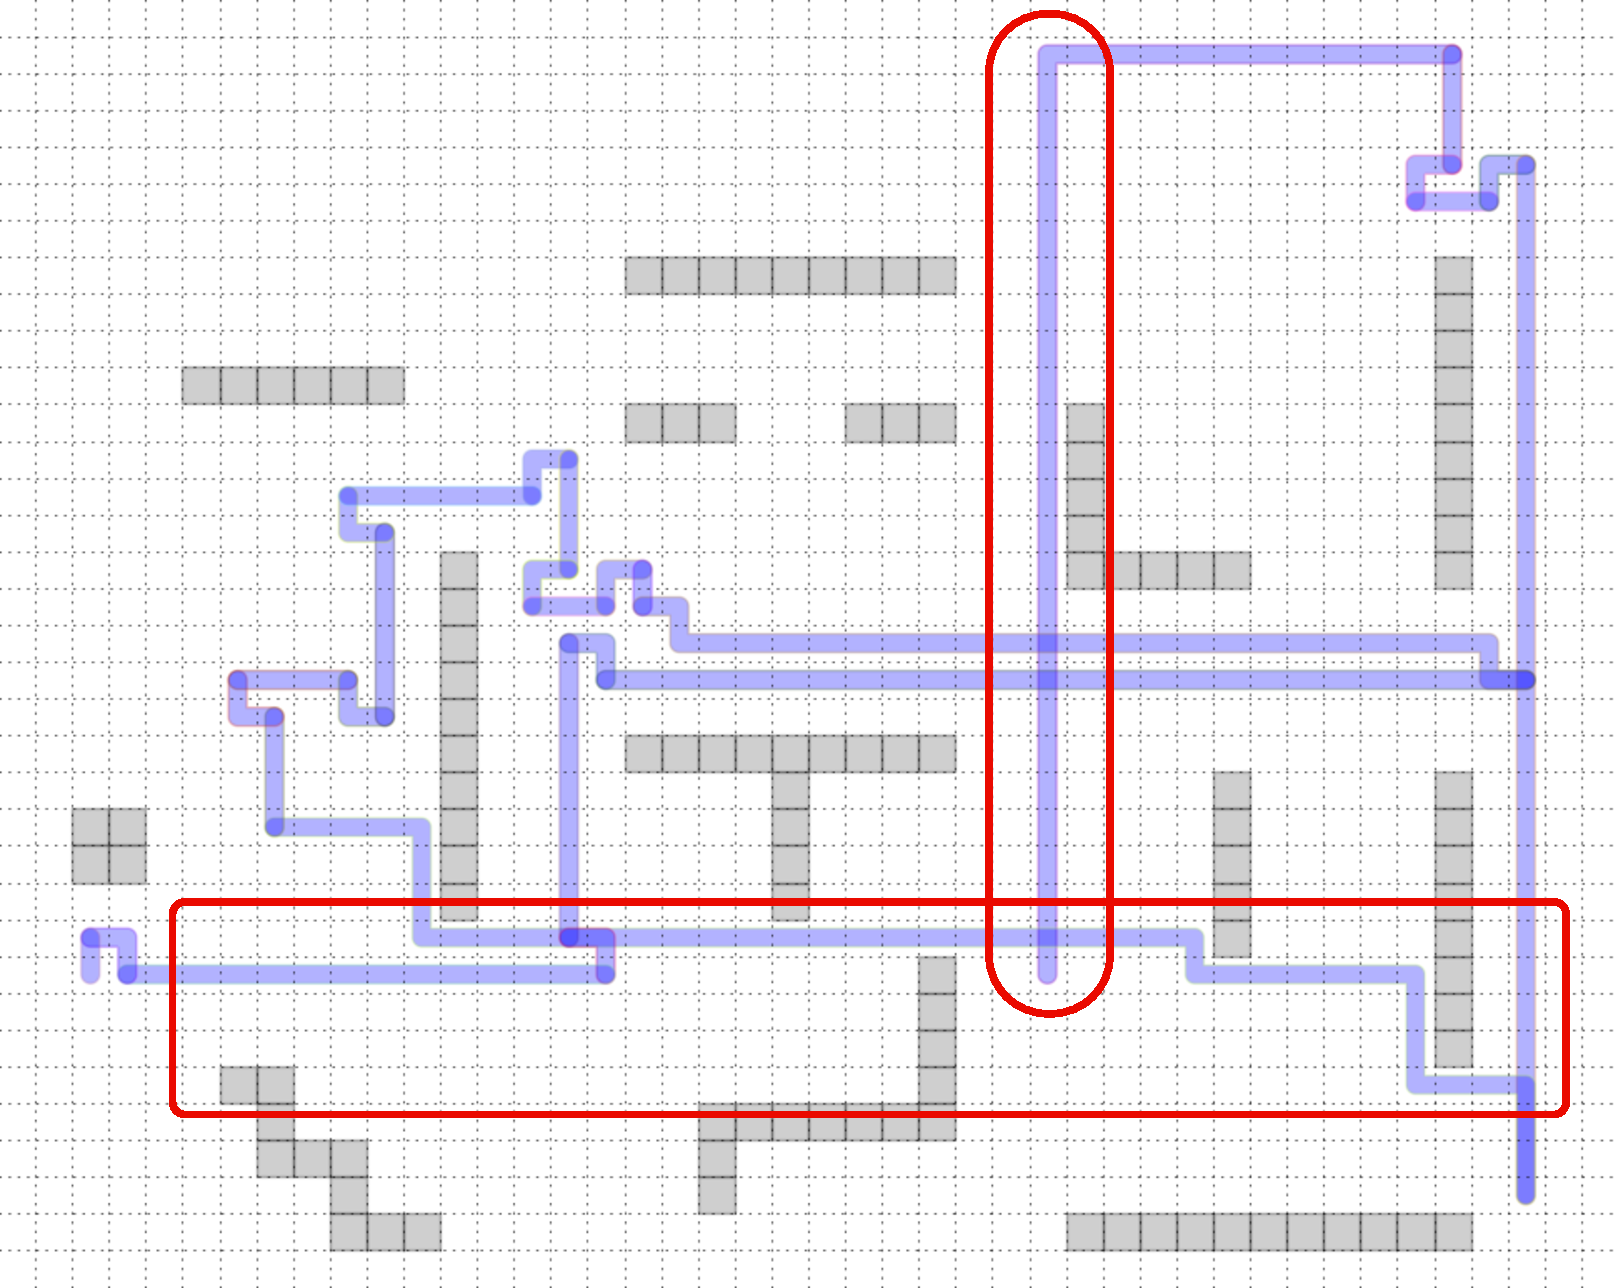
\includegraphics[width=0.7\textwidth, height=0.7\textwidth]{imgs/experimentos/figure_simple.pdf}}
                % \vspace{0.6cm}
                \caption*{\centering Tipo de Transporte}
            \end{subfigure}
            \begin{subfigure}[b]{0.32\textwidth}
                \centering
                \fbox{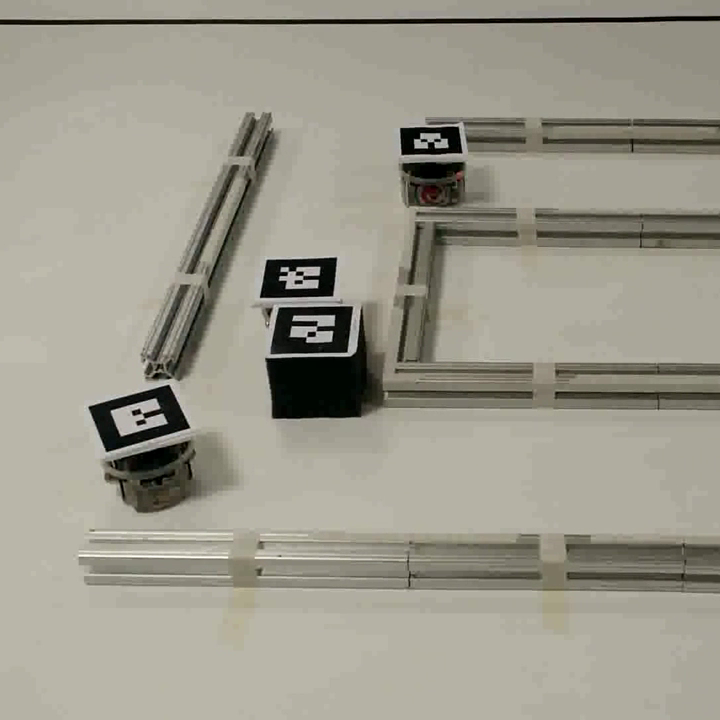
\includegraphics[width=0.7\textwidth]{imgs/experimentos/real.png}}
                \caption*{\centering Ambiente Real}
            \end{subfigure}
            % \begin{subfigure}[b]{0.24\textwidth}
            %     \fbox{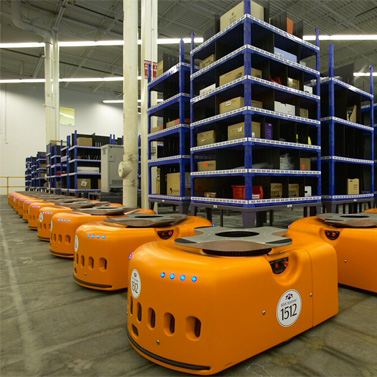
\includegraphics[width=\textwidth]{imgs/transporte1.png}}
            %     \caption*{Transporte}
            % \end{subfigure}
        \end{figure}

            % \begin{column}[c]{0.3\textwidth}
            %     \begin{figure}[p]
            %         \centering
            %         \setlength{\fboxsep}{0pt}
            %         \fbox{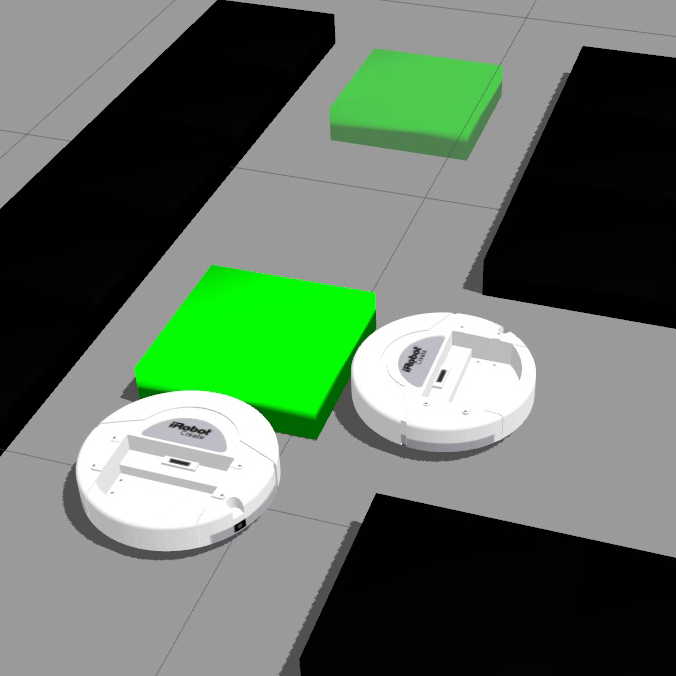
\includegraphics[width=0.9\textwidth]{imgs/experimentos/sim.png}}
            %         \caption*{\centering Simulação}
            %     \end{figure}
            % \end{column}

    }

    % \frame{
        % OUT
        % \frametitle{Experimentos}

        % \begin{columns}[c]
        %     \begin{column}[c]{0.3\textwidth}
        %         \begin{figure}[p]
        %             \centering
        %             \setlength{\fboxsep}{0pt}
        %             \fbox{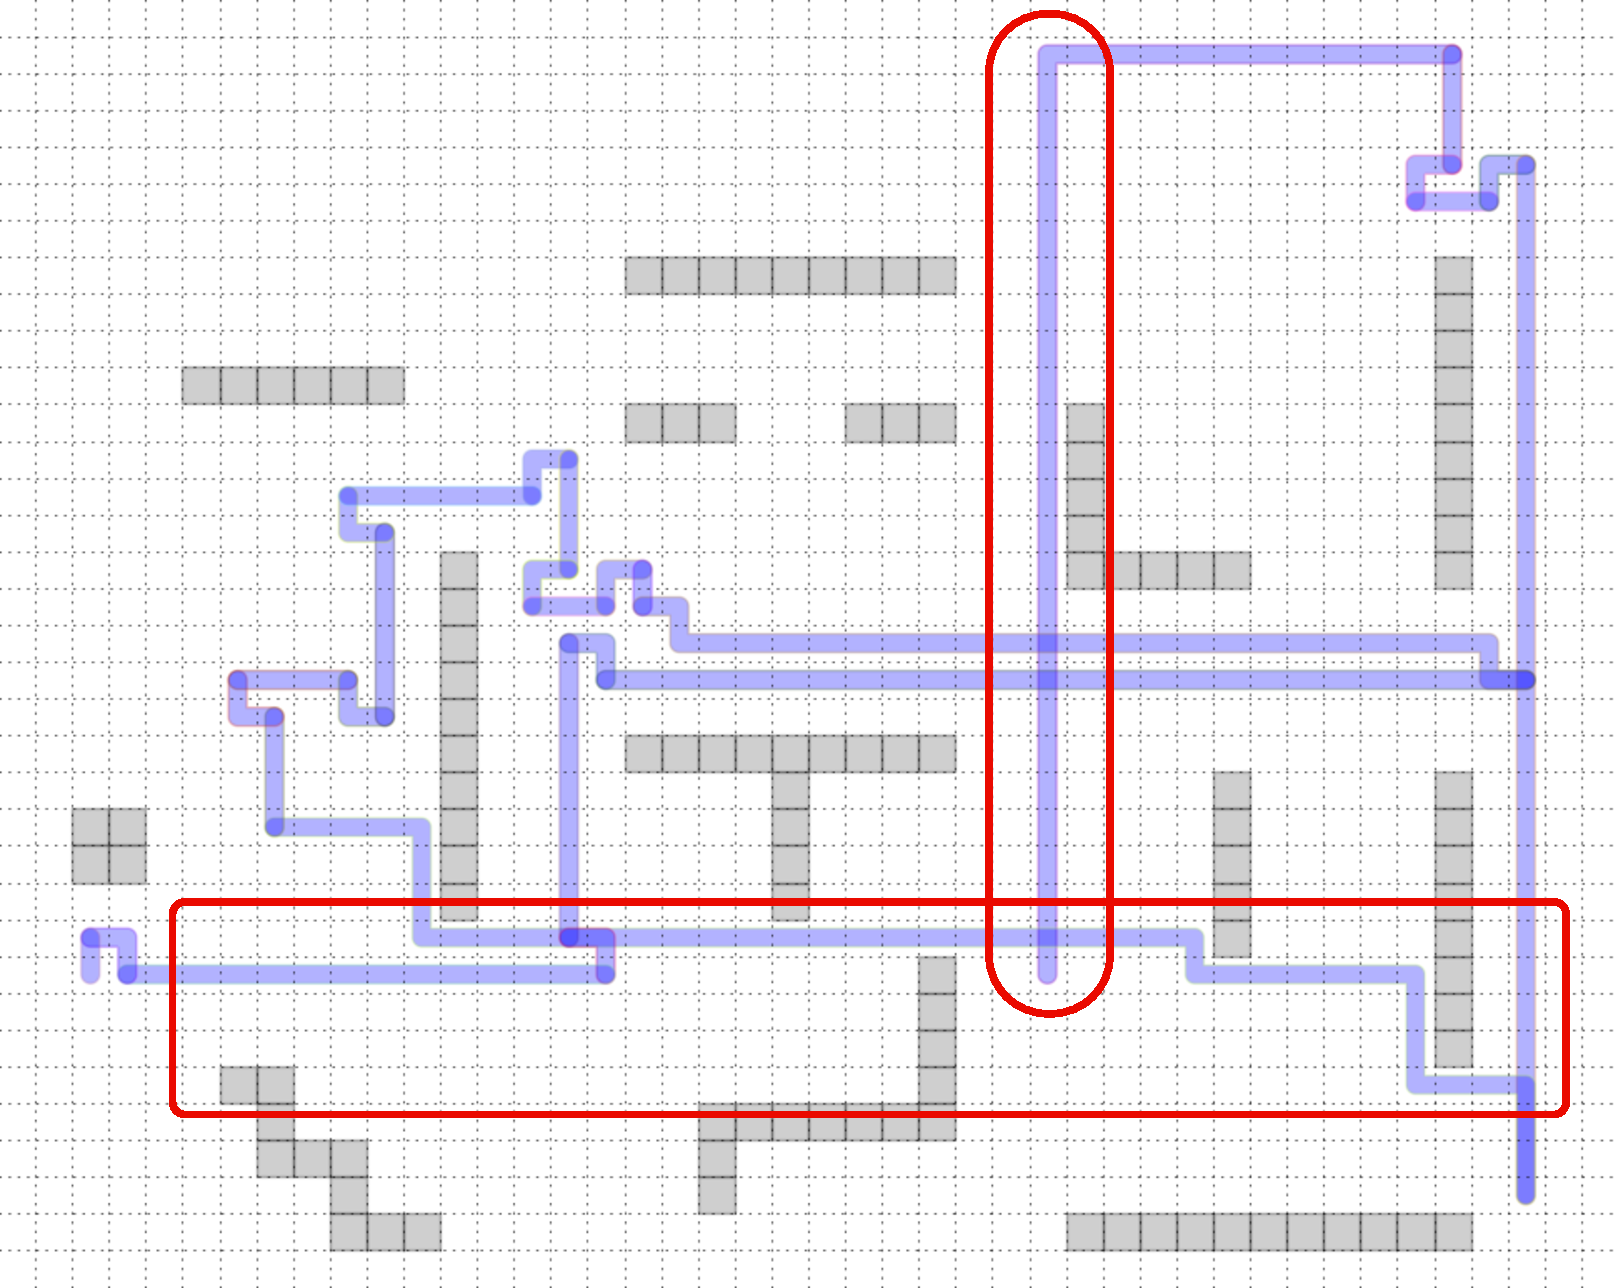
\includegraphics[width=0.9\textwidth]{imgs/experimentos/figure_simple.pdf}}
        %             \vspace{0.6cm}
        %             \caption*{\centering Sequenciamento}
        %         \end{figure}
        %     \end{column}
        %     \begin{column}[c]{0.3\textwidth}
        %         \begin{figure}[p]
        %             \centering
        %             \setlength{\fboxsep}{0pt}
        %             \fbox{\includegraphics[width=0.9\textwidth]{imgs/experimentos/sim.png}}
        %             \caption*{\centering Simulação}
        %         \end{figure}
        %     \end{column}
        %     \begin{column}[c]{0.3\textwidth}
        %         \begin{figure}[p]
        %             \centering
        %             \setlength{\fboxsep}{0pt}
        %             \fbox{\includegraphics[width=0.9\textwidth]{imgs/experimentos/real.png}}
        %             \caption*{\centering Ambiente Real}
        %         \end{figure}
        %     \end{column}
        % \end{columns}
    % }

    \frame{
        \frametitle{Experimentos}
        \framesubtitle{Complexidade do Mapa}

        Ambiente variável em complexidade, sempre com 3 objetos e 3 agentes.

        \begin{columns}[c]
            \begin{column}[c]{0.24\textwidth}
                \begin{figure}[p]
                    \centering
                    \includegraphics[width=\textwidth]{imgs/experimentos/ambient_1.png}
                    \caption*{\centering Sem obstáculos no ambiente}
                \end{figure}
            \end{column}
            \begin{column}[c]{0.24\textwidth}
                \begin{figure}[p]
                    \centering
                    \includegraphics[width=\textwidth]{imgs/experimentos/ambient_2.png}
                    \caption*{\centering Obstáculos dispersos}
                \end{figure}
            \end{column}
            \begin{column}[c]{0.24\textwidth}
                \begin{figure}[p]
                    \centering
                    \includegraphics[width=\textwidth]{imgs/experimentos/ambient_3.png}
                    \caption*{\centering Pequena restrição de movimento}
                \end{figure}
            \end{column}
            \begin{column}[c]{0.24\textwidth}
                \begin{figure}[p]
                    \centering
                    \includegraphics[width=\textwidth]{imgs/experimentos/ambient_4.png}
                    \caption*{\centering Grande restrição de movimento}
                \end{figure}
            \end{column}
        \end{columns}
    }

    % \frame{
    %     \frametitle{Experimentos}
    %     \framesubtitle{Complexidade do Mapa}

    %     Deslocamento do Objeto:

    %     \begin{figure}[p]
    %         \centering
    %         \includegraphics[width=0.8\textwidth]{imgs/experimentos/ambient_objeto.png}
    %     \end{figure}
    % }

    % \frame{
    %     \frametitle{Experimentos}
    %     \framesubtitle{Complexidade do Mapa}

    %     Deslocamento dos Agentes:

    %     \begin{figure}[p]
    %         \centering
    %         \includegraphics[width=0.8\textwidth]{imgs/experimentos/ambient_robo.png}
    %     \end{figure}
    % }

    \frame{
        \frametitle{Experimentos}
        \framesubtitle{Complexidade do Mapa}

        Tempo de Planejamento:

        \begin{figure}[p]
            \centering
            \includegraphics[width=0.8\textwidth]{imgs/experimentos/ambient_tempo.png}
        \end{figure}
    }

    \frame{
        \frametitle{Experimentos}
        \framesubtitle{Penalização da mudança de direção}

        Ambiente fixo, número de objetos e agentes variável.

        \begin{figure}[p]
            \centering
            \includegraphics[width=0.6\textwidth]{imgs/experimentos/ambiente_penalizado.png}
        \end{figure}
    }

    \frame{
        \frametitle{Experimentos}
        \framesubtitle{Penalização da mudança de direção}

        \begin{columns}[c]
            \begin{column}[c]{0.5\textwidth}
                \begin{figure}[p]
                    \centering
                    \setlength{\fboxsep}{0pt}
                    \fbox{\includegraphics[width=0.9\textwidth]{imgs/experimentos/ambiente_penalizacao_sem.pdf}}
                    \caption*{\centering Sem penalização}
                \end{figure}
            \end{column}
            \begin{column}[c]{0.5\textwidth}
                \begin{figure}[p]
                    \centering
                    \setlength{\fboxsep}{0pt}
                    \fbox{\includegraphics[width=0.9\textwidth]{imgs/experimentos/ambiente_penalizacao_com.pdf}}
                    \caption*{\centering Com penalização}
                \end{figure}
            \end{column}
        \end{columns}
    }

    % \frame{
        % OUT
        % \frametitle{Experimentos}
        % \framesubtitle{Penalização da mudança de direção}

        % Deslocamento dos agentes:

        % \begin{columns}[c]
        %     \begin{column}[c]{0.5\textwidth}
        %         \begin{figure}[p]
        %             \centering
        %             \setlength{\fboxsep}{0pt}
        %             \fbox{\includegraphics[width=0.9\textwidth]{imgs/experimentos/penalizacao/penalizado_des_sem_1_4.png}}
        %             \caption*{\centering Sem penalização}
        %         \end{figure}
        %     \end{column}
        %     \begin{column}[c]{0.5\textwidth}
        %         \begin{figure}[p]
        %             \centering
        %             \setlength{\fboxsep}{0pt}
        %             \fbox{\includegraphics[width=0.9\textwidth]{imgs/experimentos/penalizacao/penalizado_des_com_1_4.png}}
        %             \caption*{\centering Com penalização}
        %         \end{figure}
        %     \end{column}
        % \end{columns}
    % }

    \frame{
        \frametitle{Experimentos}
        \framesubtitle{Penalização da mudança de direção}

        Deslocamento dos agentes:

        \begin{columns}[c]
            \begin{column}[c]{0.5\textwidth}
                \begin{figure}[p]
                    \centering
                    \setlength{\fboxsep}{0pt}
                    \fbox{\includegraphics[width=0.9\textwidth]{imgs/experimentos/penalizacao/deslocamento_sem.png}}
                    \caption*{\centering Sem penalização}
                \end{figure}
            \end{column}
            \begin{column}[c]{0.5\textwidth}
                \begin{figure}[p]
                    \centering
                    \setlength{\fboxsep}{0pt}
                    \fbox{\includegraphics[width=0.9\textwidth]{imgs/experimentos/penalizacao/deslocamento_com.png}}
                    \caption*{\centering Com penalização}
                \end{figure}
            \end{column}
        \end{columns}
    }

    % \frame{
        % OUT
        % \frametitle{Experimentos}
        % \framesubtitle{Penalização da mudança de direção}

        % Tempo de Planejamento:

        % \begin{columns}[c]
        %     \begin{column}[c]{0.5\textwidth}
        %         \begin{figure}[p]
        %             \centering
        %             \setlength{\fboxsep}{0pt}
        %             \fbox{\includegraphics[width=0.9\textwidth]{imgs/experimentos/penalizacao/penalizado_tem_sem_1_4.png}}
        %             \caption*{\centering Sem penalização}
        %         \end{figure}
        %     \end{column}
        %     \begin{column}[c]{0.5\textwidth}
        %         \begin{figure}[p]
        %             \centering
        %             \setlength{\fboxsep}{0pt}
        %             \fbox{\includegraphics[width=0.9\textwidth]{imgs/experimentos/penalizacao/penalizado_tem_com_1_4.png}}
        %             \caption*{\centering Com penalização}
        %         \end{figure}
        %     \end{column}
        % \end{columns}
    % }

    \frame{
        \frametitle{Experimentos}
        \framesubtitle{Penalização da mudança de direção}

        Tempo de Planejamento:

        \begin{columns}[c]
            \begin{column}[c]{0.5\textwidth}
                \begin{figure}[p]
                    \centering
                    \setlength{\fboxsep}{0pt}
                    \fbox{\includegraphics[width=0.9\textwidth]{imgs/experimentos/penalizacao/tempo_sem.png}}
                    \caption*{\centering Sem penalização}
                \end{figure}
            \end{column}
            \begin{column}[c]{0.5\textwidth}
                \begin{figure}[p]
                    \centering
                    \setlength{\fboxsep}{0pt}
                    \fbox{\includegraphics[width=0.9\textwidth]{imgs/experimentos/penalizacao/tempo_com.png}}
                    \caption*{\centering Com penalização}
                \end{figure}
            \end{column}
        \end{columns}
    }

    \frame{
        \frametitle{Experimentos}
        \framesubtitle{Função de Utilidade}

        Para demonstrar a flexibilidade do sistema, foram utilizado diferentes pesos na função de utilidade.

        \begin{equation*}
            \utilityfunction(\type{i}, \movementaction) = \alpha \cdot \timefunction(\type{i}, \movementaction) + (1 - \alpha) \cdot \energyfunction(\type{i}, \movementaction)
        \end{equation*}

        \begin{table}
            \centering
            \begin{tabular}{|c|c|c|}
            \hline
            Experimento & Deslocamento ($\alpha$) & Energia ($1 - \alpha$) \\ \hline
            1        & 1     & 0       \\ \hline
            2        & 0     & 1       \\ \hline
            3        & 0.5   & 0.5     \\ \hline
            \end{tabular}
        \end{table}
    }

    \frame{
        \frametitle{Experimentos}
        \framesubtitle{Função de Utilidade}

        \begin{columns}[c]
            \begin{column}[c]{0.33\textwidth}
                \begin{figure}[p]
                    \centering
                    \setlength{\fboxsep}{0pt}
                    \fbox{\includegraphics[width=\textwidth]{imgs/experimentos/utility_func_time.png}}
                    \caption*{\centering Experimento 1 Deslocamento}
                \end{figure}
            \end{column}
            \begin{column}[c]{0.33\textwidth}
                \begin{figure}[p]
                    \centering
                    \setlength{\fboxsep}{0pt}
                    \fbox{\includegraphics[width=\textwidth]{imgs/experimentos/utility_func_energy.png}}
                    \caption*{\centering Experimento 2\hspace{\textwidth} Energia}
                \end{figure}
            \end{column}
            \begin{column}[c]{0.33\textwidth}
                \begin{figure}[p]
                    \centering
                    \setlength{\fboxsep}{0pt}
                    \fbox{\includegraphics[width=\textwidth]{imgs/experimentos/utility_func_mid.png}}
                    \caption*{\centering Experimento 3 Balanceado}
                \end{figure}
            \end{column}
        \end{columns}
    }

    \frame{
        \frametitle{Experimentos}
        \framesubtitle{Tipo de Transporte}

        Somente um agente responsável pelo transporte de vários objetos.

        \begin{figure}[p]
            \centering
            \includegraphics[width=0.6\textwidth]{imgs/experimentos/mapa_sequencial_oportunista.png}
        \end{figure}
    }

    \frame{
        \frametitle{Experimentos}
        \framesubtitle{Tipo de Transporte}

        \begin{columns}[c]
            \begin{column}[c]{0.5\textwidth}
                \begin{figure}[p]
                    \centering
                    \setlength{\fboxsep}{0pt}
                    \fbox{\includegraphics[width=0.9\textwidth]{imgs/experimentos/figure_simple.pdf}}
                    \caption*{\centering Sequencial}
                \end{figure}
            \end{column}
            \begin{column}[c]{0.5\textwidth}
                \begin{figure}[p]
                    \centering
                    \setlength{\fboxsep}{0pt}
                    \fbox{\includegraphics[width=0.9\textwidth]{imgs/experimentos/figure_smart.pdf}}
                    \caption*{\centering Oportunista}
                \end{figure}
            \end{column}
        \end{columns}
    }

    \frame{
        \frametitle{Experimentos}
        \framesubtitle{Tipo de Transporte}

        Deslocamento do agente:

        \begin{figure}[p]
            \centering
            \includegraphics[width=0.7\textwidth]{imgs/experimentos/sequencial_oportunista_deslocamento.png}
        \end{figure}
    }

    \frame{
        \frametitle{Experimentos}
        \framesubtitle{Tipo de Transporte}

        Tempo de planejamento:

        \begin{figure}[p]
            \centering
            \includegraphics[width=0.7\textwidth]{imgs/experimentos/sequencial_oportunista_tempo.png}
        \end{figure}
    }

    % \frame{
        % OUT
        % \frametitle{Experimentos}
        % \framesubtitle{Ambiente Simulado}

        % \begin{figure}[p]
        %     \centering
        %     \fbox{\movie[height=0.5\textwidth, width=0.9\textwidth, autostart, loop]{}{newvideo.ogv}}
        % \end{figure}
    % }

    \frame{
        \frametitle{Experimentos}
        \framesubtitle{Ambiente Real}

        \begin{figure}[p]
            \centering
            \fbox{\movie[height=0.5\textwidth, width=0.9\textwidth, autostart, loop]{}{transport_video.mp4}}
        \end{figure}
    }

    % section experimentos (end)

    \section{Conclusão e Trabalhos Futuros} % (fold)
    \label{sec:conclus_o}

    \frame{
        \frametitle{Conclusão}

        \begin{block}{}
            \justify
            Este trabalho apresenta uma metodologia para o transporte de objetos utilizando uma equipe de agentes heterogêneos capaz de tratar todas as etapas da manipulação:
            % , demonstrando um conjunto de técnicas capaz de tratar o problema de forma completa, desde o planejamento da movimentação dos objetos até a execução pelos agentes.
        \end{block}

        \vspace{0.2cm}
        % Foram tratados os problemas:
        \begin{enumerate}
            \item Planejamento para os Objetos;
            \item Alocação de Tarefas entre a equipe;
            \item Coordenação e execução do transporte.
        \end{enumerate}

        % \begin{block}{}
        %     \justify
        %     O sistema é flexível, pois consegue atender a diferentes demandas, como um transporte mais rápido, ou que economize energia.
        %     Além de ser capaz de utilizar os agentes disponíveis para melhorar o transporte de forma geral.
        % \end{block}

        \begin{block}{Publicação}
            \emph{Multi-object Transportation using a Mobile Robot}\\
            Melo, R. S., Macharet, D. G., e Campos, M. F. M.\\
            LARS 2015 -- \emph{12th Latin American Robotics Symposium}
        \end{block}
    }

    % \frame{
        % OUT
        % \frametitle{Conclusão}

        % \begin{block}{}
        %     \justify
        %     O sistema é flexível, no sentido de poder atender a certas demandas, como um transporte mais rápido, ou que economize energia.
        %     Além de ser capaz de utilizar os agentes disponíveis para melhorar o transporte de forma geral.
        % \end{block}

        % \begin{block}{}

        % \end{block}
    % }

    \frame{
        \frametitle{Trabalhos Futuros}

        Algumas extensões que podem ser aplicada ao sistema demonstrado:

        \begin{itemize}
            \item Módulo de exploração e mapeamento do ambiente;
            \item Utilização de agente aéreo para localização dos demais robôs;
            \item Transporte cooperativo simultâneo;
            \item Colaboração entre robôs e humanos.
        \end{itemize}
    }

    \frame[plain]{
        % \frametitle{}
        \centering
        {\huge\textsc{Obrigado}}

        \vspace{1cm}

        {\huge\textsc{Perguntas?}}

        \vspace{1.6cm}

        \includegraphics[height=0.2\textheight]{imgs/capes.png}
        \hspace{0.6cm}
        \includegraphics[height=0.2\textheight]{imgs/cnpq.jpg}
        \hspace{0.6cm}
        \includegraphics[height=0.2\textheight]{imgs/fapemig.png}

        % \begin{columns}[T]
        %     \begin{column}[T]{0.5\textwidth}
        %         Obrigado
        %     \end{column}
        %     \begin{column}[T]{0.5\textwidth}
        %     \end{column}
        % \end{columns}
    }

    % section conclus_o (end)

    \section{Bibliografia} % (fold)
    \label{sec:bibliografia}

    \backupbegin
    \begin{frame}[allowframebreaks]
        \frametitle{References}

        \bibliographystyle{apalike}
        % \printbibliography
        \footnotesize
        \bibliography{references.bib}

    \end{frame}
    \backupend

    % section bibliografia (end)

\end{document}
